% =====================================================================
%  BÁO CÁO ĐỒ ÁN KHOA HỌC
%  Nghiên cứu và ứng dụng mô hình Dual Agreement Consistency Learning
%  cho bài toán phân đoạn tế bào máu trong ảnh hiển vi
%  Biên dịch: pdfLaTeX + BibTeX  (latexmk -pdf report.tex)
%  Các bảng trong thư mục tables/ được sinh tự động từ thư mục results/.
% =====================================================================
\documentclass[12pt,a4paper,oneside]{report}

% ---------- Tiếng Việt ----------
\usepackage[T5]{fontenc}
\usepackage[utf8]{inputenc}
\usepackage[vietnamese]{babel}
\usepackage{lmodern}

% ---------- Trình bày ----------
\usepackage[left=3cm,right=2cm,top=2.5cm,bottom=2.5cm]{geometry}
\usepackage{setspace}\onehalfspacing
\usepackage{indentfirst}
\setlength{\parindent}{1cm}
\setlength{\parskip}{4pt}
\usepackage{titlesec}
\usepackage{enumitem}
\setlist{nosep,leftmargin=*}

\titleformat{\chapter}[display]
  {\normalfont\bfseries\centering}
  {\large\MakeUppercase{\chaptertitlename}\ \thechapter}{4pt}{\Large}
\titlespacing*{\chapter}{0pt}{-10pt}{20pt}
\titleformat{\section}{\normalfont\large\bfseries}{\thesection}{0.6em}{}
\titleformat{\subsection}{\normalfont\normalsize\bfseries}{\thesubsection}{0.6em}{}

% ---------- Toán, bảng, hình ----------
\usepackage{amsmath,amssymb,bm}
\usepackage{booktabs,tabularx,multirow,array}
\usepackage{graphicx}
\usepackage{xcolor}
\usepackage{tikz}
\usetikzlibrary{positioning,arrows.meta,fit,calc}
\usepackage{caption}
\captionsetup{font=small,labelfont=bf}
\usepackage{float}
\usepackage[hidelinks]{hyperref}
\graphicspath{{figures/}}

\newcommand{\Lsup}{\mathcal{L}_{\mathrm{sup}}}
\newcommand{\Lcps}{\mathcal{L}_{\mathrm{cps}}}
\newcommand{\Lict}{\mathcal{L}_{\mathrm{ict}}}
\newcommand{\Ldac}{\mathcal{L}_{\mathrm{dac}}}
\newcommand{\Lkl}{\mathcal{L}_{\mathrm{KL}}}
\newcommand{\Lent}{\mathcal{L}_{\mathrm{ent}}}
\newcommand{\JSD}{\mathrm{JSD}}
\newcommand{\KL}{\mathrm{KL}}

% Nạp các dòng bảng sinh tự động bên trong môi trường tabular.
% \input của LaTeX mới chèn token ở cuối tệp làm hỏng \bottomrule, nên dùng lệnh nguyên thủy.
\makeatletter
\newcommand{\inputtable}[1]{\@@input #1 }
\makeatother

% =====================================================================
\begin{document}

% ---------------------------- TRANG BÌA -----------------------------
\begin{titlepage}
  \centering
  {\normalsize \textbf{TRƯỜNG ĐẠI HỌC CÔNG NGHIỆP THÀNH PHỐ HỒ CHÍ MINH}}\\[4pt]
  {\normalsize \textbf{KHOA CÔNG NGHỆ THÔNG TIN}}\\[2.5cm]

  {\Large \textbf{BÁO CÁO ĐỒ ÁN KHOA HỌC}}\\[1.5cm]

  {\Large \textbf{NGHIÊN CỨU VÀ ỨNG DỤNG MÔ HÌNH\\[6pt]
  {\large ``DUAL AGREEMENT CONSISTENCY LEARNING''}\\[6pt]
  CHO BÀI TOÁN PHÂN ĐOẠN TẾ BÀO MÁU\\[6pt]
  TRONG ẢNH HIỂN VI}}\\[3cm]

  \begin{tabular}{ll}
    Sinh viên thực hiện: & \underline{\hspace{6cm}} \\[4pt]
    Mã số sinh viên:     & \underline{\hspace{6cm}} \\[4pt]
    Lớp:                 & \underline{\hspace{6cm}} \\[4pt]
    Giảng viên hướng dẫn:& \underline{\hspace{6cm}} \\
  \end{tabular}

  \vfill
  {\large Thành phố Hồ Chí Minh, tháng \underline{\hspace{1cm}} năm 2026}
\end{titlepage}

\pagenumbering{roman}

% ------------------------- TRANG BẢN QUYỀN --------------------------
\thispagestyle{empty}
\vspace*{\fill}
\begin{center}
  \copyright\ 2026 \underline{\hspace{6cm}}\\[4pt]
  Bảo lưu mọi quyền.
\end{center}
\noindent Mã nguồn, cấu hình thí nghiệm và kết quả của đề tài được công bố tại\\
\url{https://github.com/duyBinh04qd/dacl-blood-cell-seg}.
Bộ dữ liệu Blood Cell Segmentation thuộc quyền của nhóm tác giả Depto và cộng sự và được sử dụng theo giấy phép MIT của kho dữ liệu gốc.
\vspace*{\fill}
\clearpage

% ---------------------------- LỜI CẢM ƠN ----------------------------
\chapter*{Lời cảm ơn}
\addcontentsline{toc}{chapter}{Lời cảm ơn}

Em xin gửi lời cảm ơn chân thành đến \underline{\hspace{5cm}}, người đã trực tiếp hướng dẫn, định hướng và góp ý cho em trong suốt quá trình thực hiện đề tài. Em cũng xin cảm ơn các thầy cô Khoa Công nghệ Thông tin, Trường Đại học Công nghiệp Thành phố Hồ Chí Minh đã trang bị cho em nền tảng kiến thức để thực hiện nghiên cứu này.

Em cảm ơn nhóm tác giả Depto và cộng sự đã công bố bộ dữ liệu Blood Cell Segmentation, cũng như các tác giả của DACL, UNeXt, Swin-Unet và các phương pháp học bán giám sát được sử dụng trong đề tài đã công khai bài báo và mã nguồn. Các thí nghiệm của đề tài được thực hiện trên tài nguyên GPU miễn phí của nền tảng Kaggle.

Do thời gian và kinh nghiệm còn hạn chế, báo cáo khó tránh khỏi thiếu sót. Em rất mong nhận được ý kiến đóng góp của thầy cô để hoàn thiện đề tài.

% ------------------------------ TÓM TẮT ------------------------------
\chapter*{Tóm tắt}
\addcontentsline{toc}{chapter}{Tóm tắt}

Phân đoạn tế bào trong ảnh hiển vi tiêu bản máu là bước nền tảng cho việc đếm và đo tế bào tự động, nhưng các mô hình học sâu cần nhiều mặt nạ được gán nhãn đến từng điểm ảnh. Đề tài xây dựng một mô hình phân đoạn bán giám sát dựa trên khung Dual Agreement Consistency Learning (DACL) của Wang và cộng sự. Mô hình huấn luyện đồng thời mạng CNN nhẹ UNeXt, mạng Transformer Swin-Unet và một giáo viên EMA của Swin-Unet, kết hợp giám sát giả chéo, nhất quán nội suy và hàm mất mát đồng thuận kép. Khi suy luận, mô hình chỉ dùng UNeXt với 1,58 triệu tham số.

Đề tài xây dựng lại từ đầu DACL cùng tám phương pháp bán giám sát tiêu biểu (MT, DCT, CPS, ICT, CTCT, PCPCS, DSTCT, LMCT) trong một khung thí nghiệm thống nhất. Các phương pháp được đánh giá trên bộ dữ liệu Blood Cell Segmentation gồm 1\,328 ảnh, ở hai mức 5\% và 10\% ảnh huấn luyện có nhãn, bằng bốn độ đo DSC, Jaccard, HD95 và ASD, cùng kiểm định Wilcoxon theo cặp. Dựa trên phân tích độ lớn của các thành phần mất mát khi mỗi vòng lặp chỉ có một ảnh có nhãn, đề tài chọn bộ trọng số $\{\lambda,\tau,\beta\}=\{0{,}2;\,0{,}2;\,1\}$.

Kết quả cho thấy DACL đạt DSC 94,38\% ở mức 5\% và 94,46\% ở mức 10\% nhãn, cao nhất trong nhóm phương pháp bán giám sát, với khác biệt có ý nghĩa thống kê so với từng phương pháp ($p<0{,}001$). Ưu thế này đến từ việc giảm đồng thời dương tính giả và âm tính giả, và tập trung ở nhóm ảnh khó nhất, nơi DACL cải thiện 1,42 điểm DSC so với UNeXt học có giám sát. Tuy nhiên, DACL không vượt rõ rệt UNeXt học có giám sát trên cùng số ảnh có nhãn, và không dẫn đầu về HD95. Nguyên nhân chính là bộ dữ liệu chỉ để lại dư địa cải thiện khoảng một điểm DSC. Đề tài cũng phân tích số hạng entropy trong hàm mất mát đồng thuận kép, và chỉ ra rằng trọng số của các thành phần không giám sát cần được chọn theo lượng tín hiệu giám sát sẵn có.

\noindent\textbf{Từ khóa:} phân đoạn ảnh y tế, tế bào máu, học bán giám sát, DACL, UNeXt, Swin-Unet.

\tableofcontents
\listoffigures
\listoftables

\chapter*{Danh mục chữ viết tắt}
\addcontentsline{toc}{chapter}{Danh mục chữ viết tắt}
\begin{center}
\small
\begin{tabularx}{\textwidth}{l X}
\toprule
Viết tắt & Ý nghĩa \\
\midrule
ASD    & Average Surface Distance -- khoảng cách bề mặt trung bình \\
CE     & Cross-Entropy -- entropy chéo \\
CNN    & Convolutional Neural Network -- mạng nơ-ron tích chập \\
CPS    & Cross Pseudo Supervision -- giám sát giả chéo \\
CTCT   & Cross Teaching between CNN and Transformer \\
DAC    & Dual-Agreement Consistency -- nhất quán đồng thuận kép \\
DACL   & Dual Agreement Consistency Learning \\
DCT    & Deep Co-Training \\
DSC    & Dice Similarity Coefficient -- hệ số tương đồng Dice \\
DSTCT  & Dual Student-Teacher framework with CNN--ViT collaborative learning \\
EMA    & Exponential Moving Average -- trung bình trượt hàm mũ \\
FS     & Fully Supervised -- học có giám sát (chỉ dùng ảnh có nhãn) \\
HD95   & 95th-percentile Hausdorff Distance -- khoảng cách Hausdorff phân vị 95 \\
ICT    & Interpolation Consistency Training -- huấn luyện nhất quán nội suy \\
JSD    & Jensen--Shannon Divergence -- độ phân kỳ Jensen--Shannon \\
KL     & Kullback--Leibler divergence -- độ phân kỳ Kullback--Leibler \\
LMCT   & phương pháp giám sát chéo CNN--Transformer của Wang, Curran và Silvestre (ISBI 2025) \\
MT     & Mean Teacher \\
PCPCS  & Pixel-level Contrastive and Pixel-level Cross-Supervised learning \\
SGD    & Stochastic Gradient Descent -- hạ gradient ngẫu nhiên \\
SSL    & Semi-Supervised Learning -- học bán giám sát \\
\bottomrule
\end{tabularx}
\end{center}

\clearpage
\pagenumbering{arabic}

% =====================================================================
\chapter{Giới thiệu}
\label{chap:gioithieu}

\section{Xác định vấn đề}

Quan sát tiêu bản máu ngoại vi dưới kính hiển vi là một xét nghiệm nền tảng trong huyết học. Từ một vi trường, kỹ thuật viên có thể đếm tế bào, đánh giá hình dạng và kích thước hồng cầu hoặc phát hiện các tế bào có hình thái bất thường. Mọi phép đo định lượng như vậy đều cần biết chính xác điểm ảnh nào thuộc tế bào và điểm ảnh nào thuộc nền. Đây chính là bài toán phân đoạn ảnh. Khi thực hiện thủ công, công việc này tốn nhiều thời gian và kết quả phụ thuộc vào người thực hiện. Vì vậy, phân đoạn tự động là bước đầu tiên của hầu hết các hệ thống phân tích ảnh tiêu bản máu.

Các mạng học sâu dạng mã hóa--giải mã, tiêu biểu là U-Net~\cite{ronneberger2015unet}, đã đạt độ chính xác cao trên bài toán này~\cite{depto2021blood}. Tuy nhiên, độ chính xác đó chỉ có được khi có đủ mặt nạ được gán nhãn đến từng điểm ảnh. Gán nhãn ảnh tế bào máu đặc biệt tốn công. Trong bộ dữ liệu mà đề tài sử dụng, mỗi mặt nạ có trung vị 56 vùng tế bào tách rời, và các tế bào chạm nhau phải được tách bằng những khe nền rộng vài điểm ảnh (mục~\ref{sec:dataset}). Trong khi đó, ảnh chưa gán nhãn có thể thu thập với số lượng lớn trong hoạt động xét nghiệm thường quy. Học bán giám sát khai thác chính sự chênh lệch này: mô hình học từ một ít ảnh có nhãn cùng nhiều ảnh không nhãn.

Dual Agreement Consistency Learning (DACL) là một khung học bán giám sát do Wang và cộng sự đề xuất~\cite{wang2026dacl}. DACL huấn luyện đồng thời một mạng CNN nhẹ (UNeXt) và một mạng Transformer (Swin-Unet). Hai mạng giám sát chéo lẫn nhau trên ảnh không nhãn, đồng thời bị ràng buộc bởi một hàm mất mát đồng thuận kép. Khi suy luận, khung này chỉ cần mạng CNN. Thiết kế đó phù hợp với mục tiêu triển khai trên thiết bị phổ thông: mô hình được hưởng lợi từ một Transformer lớn khi huấn luyện mà không phải mang theo nó khi sử dụng.

Vấn đề mà đề tài đặt ra nằm ở đặc thù của dữ liệu. DACL được xây dựng cho ảnh siêu âm thai~\cite{wang2026dacl}, nơi mỗi ảnh chứa một cấu trúc giải phẫu lớn. Ảnh hiển vi tế bào máu lại là ảnh màu nhuộm, chứa hàng chục đối tượng nhỏ trong cùng một vi trường, với nhiều tế bào chạm nhau hoặc chồng lấn. Chưa rõ các thành phần mất mát của DACL có phát huy tác dụng trên loại ảnh này hay không. Cũng chưa rõ khi so sánh trong cùng điều kiện, DACL có vượt được các phương pháp bán giám sát khác hay không, và cần cấu hình ra sao để huấn luyện ổn định khi số ảnh có nhãn rất ít.

\section{Mục đích nghiên cứu}

Mục đích của đề tài là xây dựng và đánh giá một mô hình phân đoạn tế bào máu dựa trên khung DACL khi dữ liệu có nhãn khan hiếm. Cụ thể, đề tài xây dựng lại từ đầu DACL và tám phương pháp bán giám sát tiêu biểu trong cùng một khung thí nghiệm, đánh giá chúng ở hai mức 5\% và 10\% ảnh có nhãn, và phân tích cơ chế của các thành phần mất mát để lựa chọn cấu hình phù hợp cho ảnh hiển vi. Mục tiêu sau cùng là một mô hình nhẹ, có thể triển khai trên thiết bị phổ thông, nhưng vẫn đạt độ chính xác gần với mô hình lớn.

\section{Câu hỏi nghiên cứu}
\label{sec:rq}

Đề tài trả lời ba câu hỏi nghiên cứu:
\begin{enumerate}[label=\textbf{CH\arabic*.},leftmargin=1.6cm]
  \item Ở mức 5\% và 10\% ảnh có nhãn, DACL đạt độ chính xác phân đoạn tế bào máu như thế nào so với tám phương pháp bán giám sát tiêu biểu và so với học có giám sát trên cùng số ảnh có nhãn?
  \item Lợi ích của DACL, nếu có, thể hiện ở loại lỗi nào (dương tính giả hay âm tính giả, độ trùng khớp hay độ chính xác biên) và tập trung ở những ảnh nào?
  \item Các thành phần mất mát của DACL tương tác với nhau như thế nào, và cần chọn trọng số ra sao để huấn luyện ổn định khi mỗi vòng lặp chỉ có một ảnh có nhãn?
\end{enumerate}
Câu hỏi thứ nhất và thứ hai được trả lời bằng thực nghiệm (Chương~\ref{chap:ketqua}). Câu hỏi thứ ba được trả lời bằng phân tích lý thuyết (mục~\ref{sec:loss-analysis} và~\ref{sec:weights}), kết hợp với diễn biến huấn luyện quan sát được (mục~\ref{sec:res-dynamics}).

\section{Ý nghĩa của nghiên cứu}

Về khoa học, đề tài cung cấp một đánh giá có đối chứng của DACL trên ảnh hiển vi tế bào máu. Đánh giá này dùng chung cách chia dữ liệu, tiền xử lý và chế độ huấn luyện cho mọi phương pháp, kèm kiểm định thống kê và mã nguồn có thể tái lập. Đề tài cũng phân tích số hạng entropy trong hàm mất mát đồng thuận kép. Phân tích chỉ ra rằng số hạng đó có hai tác động ngược chiều, và giải thích vì sao trọng số của nó ảnh hưởng mạnh đến độ ổn định khi huấn luyện.

Về thực tiễn, kết quả cho biết một mô hình 1,58 triệu tham số, huấn luyện với 46 ảnh có nhãn, có thể đạt độ chính xác đến đâu so với một Transformer lớn gấp 17 lần, và lợi ích đó nằm ở những loại ảnh nào. Đây là thông tin cần thiết khi quyết định có nên đầu tư gán nhãn thêm hay triển khai mô hình nhẹ cho các phòng xét nghiệm có tài nguyên tính toán hạn chế.

\section{Định nghĩa thuật ngữ}

Các thuật ngữ dưới đây được dùng thống nhất trong toàn bộ báo cáo.
\begin{description}[style=nextline,leftmargin=1cm,font=\normalfont\bfseries]
  \item[Phân đoạn ngữ nghĩa hai lớp] Gán cho mỗi điểm ảnh một trong hai nhãn \emph{tế bào} hoặc \emph{nền}, không phân biệt từng tế bào riêng lẻ.
  \item[Mặt nạ chuẩn] Mặt nạ nhị phân do con người gán nhãn, được xem là kết quả đúng khi huấn luyện và đánh giá.
  \item[Tỷ lệ nhãn] Phần trăm ảnh trong tập huấn luyện được giữ lại mặt nạ. Phần còn lại được dùng như ảnh không nhãn.
  \item[Học có giám sát (FS)] Huấn luyện chỉ trên ảnh có nhãn của một tỷ lệ nhãn cho trước, không dùng ảnh không nhãn.
  \item[Học bán giám sát (SSL)] Huấn luyện trên cả ảnh có nhãn và ảnh không nhãn, trong đó ảnh không nhãn chỉ tham gia qua các hàm mất mát không cần nhãn.
  \item[Nhãn giả] Dự đoán của một mô hình trên ảnh không nhãn, được dùng làm mục tiêu huấn luyện cho chính mô hình đó hoặc cho mô hình khác.
  \item[Giáo viên EMA] Mô hình có tham số bằng trung bình trượt hàm mũ của tham số một mô hình học sinh, dùng để sinh mục tiêu ổn định.
  \item[Ramp-up] Lịch tăng dần trọng số của các hàm mất mát không giám sát từ 0 đến giá trị tối đa trong giai đoạn đầu huấn luyện.
  \item[Thiên lệch xác nhận] Hiện tượng mô hình học theo nhãn giả sai của chính nó, hoặc của mô hình cộng tác, và ngày càng tự tin vào lỗi đó.
\end{description}

\section{Giới hạn của nghiên cứu}

Đề tài giải quyết bài toán phân đoạn ngữ nghĩa hai lớp trên ảnh hai chiều. Đề tài không phân loại các dòng tế bào và không tách từng tế bào riêng lẻ. Các phương pháp bán giám sát được đánh giá ở hai mức 5\% và 10\% nhãn, tương ứng với tình huống khan hiếm nhãn mà đề tài quan tâm. Riêng học có giám sát được chạy thêm ở mức 20\% và 100\% để xác định giới hạn trên. Do giới hạn tài nguyên tính toán, ảnh được đưa vào mạng ở độ phân giải $224\times224$, và mỗi cấu hình chỉ được huấn luyện một lần. Kết quả chỉ dựa trên một bộ dữ liệu công khai, nên chưa kiểm chứng được khả năng khái quát sang ảnh từ các phòng xét nghiệm khác.

\section{Các giả định}

Đề tài dựa trên bốn giả định. Thứ nhất, mặt nạ chuẩn của bộ dữ liệu là chính xác và nhất quán, đủ để làm cơ sở đánh giá. Thứ hai, việc ẩn mặt nạ của một phần ảnh huấn luyện mô phỏng đúng tình huống khan hiếm nhãn trong thực tế, tức là ảnh không nhãn có cùng phân phối với ảnh có nhãn. Thứ ba, tập kiểm thử 265 ảnh, được chọn ngẫu nhiên, đại diện cho phân phối của toàn bộ dữ liệu. Thứ tư, điểm số trên các ảnh kiểm thử khác nhau có thể xem là các quan sát độc lập, là điều kiện để áp dụng kiểm định Wilcoxon theo cặp.

\section{Cấu trúc của báo cáo}

Ngoài phần mở đầu, báo cáo gồm năm chương. Chương~\ref{chap:tongquan} tổng quan về bài toán phân đoạn tế bào máu, các kiến trúc mạng, học bán giám sát, các phương pháp đối chứng và mô hình DACL. Chương~\ref{chap:phuongphap} trình bày phương pháp nghiên cứu, gồm khung thực nghiệm, phân tích các thành phần mất mát và lựa chọn trọng số của DACL, cách thu thập và phân tích dữ liệu. Chương~\ref{chap:ketqua} trình bày kết quả theo từng câu hỏi nghiên cứu. Chương~\ref{chap:ketluan} tóm tắt, kết luận, thảo luận và đưa ra khuyến nghị.

% =====================================================================
\chapter{Tổng quan tài liệu và các nghiên cứu liên quan}
\label{chap:tongquan}

Chương này tổng hợp các tài liệu làm nền cho đề tài, gồm tám mục:
\begin{enumerate}[label=(\arabic*)]
  \item ảnh hiển vi tiêu bản máu và bài toán phân đoạn (mục~\ref{sec:lit-problem});
  \item kiến trúc mạng phân đoạn dạng mã hóa--giải mã (mục~\ref{sec:lit-unet});
  \item mạng UNeXt (mục~\ref{sec:lit-unext});
  \item Swin Transformer và Swin-Unet (mục~\ref{sec:lit-swin});
  \item các nguyên lý của học bán giám sát (mục~\ref{sec:ssl});
  \item tám phương pháp bán giám sát được dùng làm đối chứng (mục~\ref{sec:baselines});
  \item khung DACL (mục~\ref{sec:lit-dacl});
  \item các hàm mất mát và độ đo đánh giá (mục~\ref{sec:metrics}).
\end{enumerate}
Mục cuối chương tóm tắt các điểm chính và khoảng trống mà đề tài hướng tới.

\section{Ảnh hiển vi tiêu bản máu và bài toán phân đoạn}
\label{sec:lit-problem}

\subsection{Ảnh hiển vi tiêu bản máu ngoại vi}

Tiêu bản máu ngoại vi được tạo bằng cách dàn một giọt máu thành lớp mỏng trên lam kính, sau đó nhuộm màu để làm nổi bật tế bào. Khi chụp qua kính hiển vi quang học, mỗi ảnh là một vi trường. Trong vi trường thường có hồng cầu chiếm đa số, xen lẫn một số bạch cầu và tiểu cầu. Màu sắc và độ tương phản của ảnh phụ thuộc vào nhiều yếu tố: thuốc nhuộm và thời gian nhuộm, độ dày lớp dàn máu, nguồn sáng, cảm biến máy ảnh và cách cân bằng trắng. Vì vậy, cùng một loại tế bào có thể mang màu khá khác nhau giữa các tiêu bản hoặc giữa các phòng xét nghiệm.

Phân đoạn là bước trung gian giữa ảnh thô và các phép đo có ý nghĩa lâm sàng. Muốn đếm tế bào, đo diện tích, độ tròn hay kích thước hồng cầu, hoặc khoanh vùng để phân loại bạch cầu, trước hết phải biết vùng nào thuộc tế bào. Sai số ở bước phân đoạn truyền trực tiếp sang các phép đo phía sau. Chẳng hạn, hai tế bào bị gộp làm một sẽ làm sai số đếm, còn đường biên bị lấn ra nền sẽ làm sai diện tích đo được.

\subsection{Phát biểu bài toán và các khó khăn đặc thù}

Cho ảnh màu $x \in \mathbb{R}^{H\times W\times 3}$, bài toán phân đoạn ngữ nghĩa hai lớp yêu cầu xác định một mặt nạ $y \in \{0,1\}^{H\times W}$. Trong đó $y(u)=1$ khi điểm ảnh $u$ thuộc tế bào và $y(u)=0$ khi thuộc nền. Mô hình học sâu ước lượng phân phối xác suất lớp $p(u)$ tại từng điểm ảnh, và nhãn dự đoán là lớp có xác suất lớn nhất. Cách phát biểu này không phân biệt từng tế bào. Hai tế bào chạm nhau chỉ được tách ra nếu giữa chúng có ít nhất một dải điểm ảnh được dự đoán là nền. Bài toán tách từng đối tượng, gọi là phân đoạn thực thể, nằm ngoài phạm vi đề tài. Tuy nhiên, chất lượng phân đoạn ngữ nghĩa ở vùng tiếp giáp giữa các tế bào quyết định khả năng tách đối tượng ở bước hậu xử lý về sau.

So với phân đoạn một cấu trúc giải phẫu lớn như trong ảnh siêu âm, bài toán này có ba khó khăn đặc thù. Thứ nhất, mỗi ảnh chứa nhiều đối tượng nhỏ. Do đó, tỷ lệ điểm ảnh nằm gần đường biên lớn, và sai lệch vài điểm ảnh ở biên của mọi tế bào cộng dồn thành sai số đáng kể. Thứ hai, ở những vùng dàn máu dày, tế bào chạm nhau hoặc xếp chồng lên nhau. Ranh giới giữa chúng chỉ là những khe nền rất mảnh, khó tái tạo khi ảnh bị thu nhỏ trước khi đưa vào mạng. Thứ ba, màu sắc và chất lượng ảnh biến thiên mạnh. Ngoài ra còn có cặn thuốc nhuộm và vùng bắt màu đậm không phải tế bào. Một mô hình học từ ít ảnh có nhãn dễ khớp quá mức với điều kiện màu của chính các ảnh đó. Mục~\ref{sec:dataset} cho thấy cả ba đặc điểm này đều hiện diện rõ trong bộ dữ liệu của đề tài.

\subsection{Các hướng tiếp cận và nghiên cứu trên bộ dữ liệu}

Các phương pháp phân đoạn tế bào máu có thể chia thành ba nhóm. Nhóm xử lý ảnh truyền thống dựa trên ngưỡng hóa, phát hiện biên và thuật toán watershed. Nhóm này không cần dữ liệu huấn luyện, nhưng nhạy với tham số và với sự thay đổi màu nhuộm. Nhóm học máy cổ điển, như phân cụm điểm ảnh, vẫn dựa trên đặc trưng màu do con người lựa chọn. Nhóm học sâu tự học đặc trưng từ dữ liệu có nhãn và hiện cho độ chính xác cao nhất. Depto và cộng sự, nhóm tác giả công bố bộ dữ liệu mà đề tài sử dụng, đã so sánh cả ba nhóm~\cite{depto2021blood}. Theo trang mã nguồn công bố, nhóm học sâu gồm U-Net, U-Net++, TernausNet, Attention U-Net, R2U-Net và Attention R2U-Net. Nhóm học máy gồm ngưỡng Otsu và phân cụm K-means. Nhóm xử lý ảnh gồm watershed có điều khiển bằng điểm đánh dấu và ngưỡng hóa cân bằng histogram~\cite{depto2021repo}. Các mô hình học sâu trong so sánh đó đều được huấn luyện có giám sát. Vì vậy, chúng chịu cùng một giới hạn: cần một tập mặt nạ gán nhãn đủ lớn. Đây là điểm xuất phát của hướng học bán giám sát được trình bày ở các mục sau.

\section{Mạng phân đoạn dạng mã hóa--giải mã}
\label{sec:lit-unet}

Phần lớn các mạng phân đoạn ảnh y tế hiện nay kế thừa cấu trúc của U-Net~\cite{ronneberger2015unet}. Nhánh mã hóa giảm dần độ phân giải không gian và tăng số kênh, nhờ đó thu được đặc trưng có ngữ nghĩa cao nhưng mất thông tin vị trí chi tiết. Nhánh giải mã khôi phục dần độ phân giải để đưa ra dự đoán cho từng điểm ảnh. Điểm then chốt của U-Net là các kết nối tắt. Đặc trưng ở mỗi mức của nhánh mã hóa được ghép thẳng vào mức tương ứng của nhánh giải mã, giúp khôi phục chi tiết biên đã mất khi giảm độ phân giải. Với bài toán có nhiều đối tượng nhỏ và đường biên dày đặc như ảnh tế bào máu, kết nối tắt đặc biệt quan trọng vì phần lớn sai số nằm ở biên. Cả hai mạng trong DACL đều có dạng chữ U này. Chúng chỉ khác nhau ở cách trích xuất đặc trưng trong từng khối.

\section{Mạng UNeXt}
\label{sec:lit-unext}

UNeXt được Valanarasu và Patel đề xuất nhằm phân đoạn ảnh y tế với chi phí tính toán thấp~\cite{valanarasu2022unext}. Mạng giữ cấu trúc chữ U nhưng chia nhánh mã hóa thành hai giai đoạn. Ba tầng đầu là khối tích chập thông thường, làm việc ở độ phân giải cao, nơi tích chập trích xuất đặc trưng cục bộ hiệu quả. Hai tầng sau, ở độ phân giải thấp, thay tích chập bằng khối MLP mã hóa token (tokenized MLP). Trong khối này, bản đồ đặc trưng được dịch chuyển theo chiều rộng hoặc chiều cao trước khi đi qua lớp MLP. Nhờ phép dịch, mỗi token tiếp nhận thông tin từ các vị trí lân cận mà không cần cơ chế tự chú ý tốn kém. Một lớp tích chập theo chiều sâu xen giữa các lớp MLP đảm nhiệm việc mã hóa thông tin vị trí. Nhánh giải mã đối xứng với nhánh mã hóa và cũng dùng kết nối tắt. Đề tài dùng cấu hình số kênh $\{32,64,128,160,256\}$ cho nhánh mã hóa, như trong khung DACL~\cite{wang2026dacl}. Số tham số và số phép tính của cấu hình này được trình bày ở mục~\ref{sec:complexity}.

\section{Swin Transformer và Swin-Unet}
\label{sec:lit-swin}

Transformer dựa trên cơ chế tự chú ý~\cite{vaswani2017attention}: mỗi token được cập nhật bằng tổ hợp có trọng số của mọi token khác. Cơ chế này cho phép mô hình hóa quan hệ ở khoảng cách xa, nhưng chi phí tăng theo bình phương số token, nên không khả thi khi áp dụng trực tiếp lên ảnh độ phân giải cao. Swin Transformer giải quyết vấn đề bằng cách chỉ tính tự chú ý trong các cửa sổ cục bộ không chồng lấn, mỗi cửa sổ gồm $M\times M$ token~\cite{liu2021swin}. Giữa hai khối liên tiếp, lưới cửa sổ được dịch đi $\lfloor M/2\rfloor$ token để thông tin truyền được qua ranh giới cửa sổ. Sau mỗi giai đoạn, phép gộp token ghép bốn token kề nhau thành một, tạo ra biểu diễn phân cấp tương tự nhánh mã hóa của CNN. Chi phí tính toán nhờ đó chỉ tăng tuyến tính theo kích thước ảnh.

Swin-Unet xây dựng cấu trúc chữ U hoàn toàn bằng các khối Swin Transformer~\cite{cao2022swinunet}. Ảnh được cắt thành các ô $4\times4$ và chiếu thành token 96 chiều. Nhánh mã hóa gồm ba giai đoạn với số chiều đặc trưng 96, 192 và 384, tiếp theo là tầng thắt cổ chai 768 chiều. Nhánh giải mã dùng phép mở rộng token, ngược với phép gộp, để tăng độ phân giải, và nhận kết nối tắt từ nhánh mã hóa. Đề tài dùng phiên bản \emph{tiny} với kích thước cửa sổ $M=7$, khởi tạo nhánh mã hóa từ trọng số Swin-T đã huấn luyện trên ImageNet-1K~\cite{deng2009imagenet}.

Lý do ghép một CNN với một Transformer đã được Luo và cộng sự phân tích. CNN thiên về đặc trưng cục bộ, còn Transformer nắm bắt tốt hơn quan hệ ở khoảng cách xa. Vì vậy, hai loại mạng thường mắc lỗi ở những vị trí khác nhau, và dự đoán của mạng này có thể bổ khuyết cho mạng kia khi giám sát chéo~\cite{luo2022ctct}.

\section{Học bán giám sát}
\label{sec:ssl}

\subsection{Bài toán và các giả định}

Trong học bán giám sát cho phân đoạn, tập huấn luyện gồm tập có nhãn $\mathcal{D}_L=\{(x_i,y_i)\}_{i=1}^{N}$ và tập không nhãn $\mathcal{D}_U=\{u_j\}_{j=1}^{M}$, thường với $M\gg N$. Hàm mục tiêu có dạng chung
\begin{equation}
  \mathcal{L} = \Lsup(\mathcal{D}_L) + w(t)\,\mathcal{L}_{\mathrm{unsup}}(\mathcal{D}_U),
  \label{eq:ssl}
\end{equation}
trong đó $\mathcal{L}_{\mathrm{unsup}}$ không dùng nhãn và $w(t)$ là trọng số có thể thay đổi theo vòng lặp $t$. Ảnh không nhãn chỉ hữu ích khi phân phối của chúng chứa thông tin về ranh giới quyết định. Điều này được phát biểu qua các giả định cơ bản~\cite{chapelle2006ssl,vanengelen2020survey}. Giả định trơn cho rằng hai điểm gần nhau trong vùng dữ liệu dày đặc nên có cùng nhãn. Giả định cụm, hay giả định mật độ thấp, cho rằng ranh giới quyết định nên đi qua vùng ít dữ liệu. Với ảnh tế bào máu, giả định cụm khá hợp lý ở cấp điểm ảnh, vì phần lớn điểm ảnh thuộc tế bào hoặc thuộc nền một cách rõ ràng. Ngược lại, giả định này yếu đi ở vùng tiếp giáp giữa các tế bào, nơi các khe nền mảnh mang ít tín hiệu thị giác.

\subsection{Chính quy hóa nhất quán và mô hình giáo viên}

Nhóm phương pháp chính quy hóa nhất quán buộc mô hình đưa ra dự đoán ổn định khi đầu vào hoặc tham số bị nhiễu. Theo giả định trơn, một dự đoán đúng không nên thay đổi trước những nhiễu không làm đổi nội dung ảnh. Mean Teacher~\cite{tarvainen2017mt} tạo mục tiêu nhất quán từ một mô hình giáo viên, có tham số là trung bình trượt hàm mũ của tham số mô hình học sinh: $\bar\theta \leftarrow \alpha\bar\theta + (1-\alpha)\theta$. Vì là trung bình theo thời gian, giáo viên dao động ít hơn học sinh và cho mục tiêu ổn định hơn.

Ở đầu quá trình huấn luyện, dự đoán trên ảnh không nhãn gần như ngẫu nhiên, nên ép mô hình nhất quán với chúng có thể gây hại. Vì vậy, nhiều phương pháp tăng dần trọng số $w(t)$ theo hàm ramp-up dạng sigmoid $w(t)=w_{\max}\exp\!\big(-5(1-t/T)^2\big)$ với $t\le T$~\cite{laine2017temporal}. Trong mã nguồn bán giám sát phổ biến cho ảnh y tế SSL4MIS, trọng số nhất quán mặc định là $w_{\max}=0{,}1$ và cũng được tăng theo ramp-up~\cite{luo2020ssl4mis}.

\subsection{Nhãn giả, cực tiểu hóa entropy và thiên lệch xác nhận}

Một hướng khác là dùng chính dự đoán của mô hình trên ảnh không nhãn làm nhãn giả để huấn luyện tiếp. Grandvalet và Bengio chỉ ra rằng việc cực tiểu hóa entropy của dự đoán trên dữ liệu không nhãn đẩy ranh giới quyết định ra khỏi vùng dữ liệu dày đặc, tức là thực hiện giả định cụm~\cite{grandvalet2005entropy}. Huấn luyện bằng nhãn giả cứng (one-hot) có tác dụng tương tự. Mặt trái của cả hai cơ chế là thiên lệch xác nhận~\cite{arazo2020pseudo}. Nếu mô hình đã sai ở một vùng, nhãn giả sinh ra từ dự đoán sai sẽ củng cố chính lỗi đó. Rủi ro này càng lớn khi tập có nhãn nhỏ, vì tín hiệu giám sát thật không đủ mạnh để kéo mô hình trở lại.

\subsection{Đồng huấn luyện với hai mạng}

Để giảm thiên lệch xác nhận, nhóm phương pháp đồng huấn luyện dùng hai mạng sinh nhãn giả cho nhau thay vì cho chính mình. Khi hai mạng mắc lỗi ở những vị trí khác nhau, mỗi mạng có cơ hội được mạng kia sửa sai. Hiệu quả của cơ chế này phụ thuộc vào mức độ khác biệt giữa hai mạng. Nếu hai mạng hội tụ về cùng một lời giải, chúng sẽ củng cố lỗi của nhau giống như một mạng tự huấn luyện. Vì vậy, một số phương pháp chủ động duy trì sự khác biệt, bằng ví dụ đối kháng như DCT~\cite{qiao2018dct} hoặc bằng kiến trúc dị thể như các phương pháp CNN--Transformer~\cite{luo2022ctct}.

\section{Các phương pháp học bán giám sát tiêu biểu}
\label{sec:baselines}

Đề tài chọn tám phương pháp bán giám sát tiêu biểu, công bố từ năm 2017 đến 2025, làm đối chứng. Tám phương pháp này đại diện cho ba hướng tiếp cận chính, từ một mạng với giáo viên EMA đến cặp mạng CNN--Transformer. Phần này trình bày ý tưởng của từng phương pháp. Cách cài đặt cụ thể trong đề tài được nêu ở mục~\ref{sec:baseline-impl}. Ký hiệu $p_i(\cdot)$ là bản đồ xác suất (softmax) của mạng thứ $i$, $\hat y_i=\arg\max p_i$ là nhãn giả cứng, và $u$ là ảnh không nhãn.

\textbf{Nhóm dùng một mạng với giáo viên EMA.} Mean Teacher (MT)~\cite{tarvainen2017mt} buộc dự đoán của học sinh trên ảnh không nhãn gần với dự đoán của giáo viên trên cùng ảnh đã thêm nhiễu: $\mathcal{L}_{\mathrm{unsup}}=\|p_\theta(u)-p_{\bar\theta}(u+\epsilon)\|^2$. Interpolation Consistency Training (ICT)~\cite{verma2022ict} thay nhiễu cộng bằng phép nội suy mixup~\cite{zhang2018mixup}. Dự đoán của học sinh trên ảnh trộn $\mathrm{Mix}_\lambda(u_0,u_1)=\lambda u_0+(1-\lambda)u_1$ phải khớp với phép trộn tương ứng của hai dự đoán từ giáo viên:
\begin{equation}
  \mathcal{L}_{\mathrm{ict}}=\big\|p_\theta(\mathrm{Mix}_\lambda(u_0,u_1))-\mathrm{Mix}_\lambda\big(p_{\bar\theta}(u_0),p_{\bar\theta}(u_1)\big)\big\|^2 ,
\end{equation}
với $\lambda$ lấy ngẫu nhiên từ phân phối Beta. Ràng buộc này buộc mô hình hành xử tuyến tính giữa các mẫu, và gián tiếp đẩy ranh giới quyết định ra khỏi vùng có mật độ dữ liệu cao.

\textbf{Nhóm dùng hai mạng cùng kiến trúc.} Deep Co-Training (DCT)~\cite{qiao2018dct} có hai thành phần. Thành phần đồng huấn luyện buộc hai mạng cùng dự đoán trên ảnh không nhãn, đo bằng độ phân kỳ Jensen--Shannon. Thành phần khác biệt góc nhìn yêu cầu mỗi mạng không bị đánh lừa bởi ví dụ đối kháng~\cite{goodfellow2015fgsm} được sinh ra để đánh lừa mạng kia. Thành phần thứ hai ngăn hai mạng sụp về cùng một lời giải. Cross Pseudo Supervision (CPS)~\cite{chen2021cps} dùng hai mạng khởi tạo khác nhau. Mỗi mạng được huấn luyện bằng nhãn giả cứng của mạng kia, không lan truyền gradient qua nhãn giả:
\begin{equation}
  \mathcal{L}_{\mathrm{cps}}=\ell\big(p_1(u),\hat y_2\big)+\ell\big(p_2(u),\hat y_1\big),
  \label{eq:cps-generic}
\end{equation}
trong đó $\ell$ là hàm mất mát phân đoạn. Cấu trúc của CPS là nền tảng của thành phần giám sát chéo trong DACL.

\textbf{Nhóm CNN--Transformer.} Phương pháp dạy chéo giữa CNN và Transformer (CTCT)~\cite{luo2022ctct} áp dụng giám sát chéo bằng nhãn giả cứng giữa một CNN và một Swin-Unet, với hàm mất mát Dice. PCPCS, viết tắt của học đối sánh và giám sát chéo ở cấp điểm ảnh, là cơ chế huấn luyện của Semi-Mamba-UNet~\cite{ma2024semimamba}. Ngoài giám sát chéo giữa một CNN và một mạng dựa trên Mamba, PCPCS thêm một thành phần đối sánh trên đầu ra đã chiếu của hai mạng. DSTCT~\cite{jiang2024dstct} dùng hai học sinh là một CNN và một ViT cùng một giáo viên EMA. Hai học sinh dạy nhau bằng cả nhãn giả cứng lẫn nhãn mềm đã làm sắc, đồng thời bị ràng buộc bởi thành phần chênh lệch độ quyết đoán giữa hai bộ phân lớp và thành phần nhất quán với giáo viên. LMCT~\cite{wang2025lmct} cũng ghép một CNN với một Transformer. Mỗi mạng học theo bản đồ xác suất mềm của mạng kia, kèm một thành phần đối sánh InfoNCE.

Xét theo trình tự thời gian, các phương pháp này phát triển theo hai hướng. Hướng thứ nhất là thay đổi nguồn tạo mục tiêu: từ nhiễu đầu vào, sang nội suy, sang mạng thứ hai, rồi sang mạng thứ hai có kiến trúc khác. Hướng thứ hai là thay đổi dạng mục tiêu: từ nhãn cứng sang nhãn mềm, kèm các ràng buộc bổ sung về phân phối hoặc đặc trưng. DACL nằm ở điểm giao của hai hướng này.

\section{Mô hình DACL}
\label{sec:lit-dacl}

DACL do Wang và cộng sự đề xuất~\cite{wang2026dacl}. Mục này trình bày kiến trúc và các hàm mất mát của khung, là cơ sở để đề tài xây dựng lại mô hình ở Chương~\ref{chap:phuongphap}.

\subsection{Kiến trúc tổng thể}

DACL gồm ba mạng (Hình~\ref{fig:dacl}). Mạng CNN $f^1_\theta$ là UNeXt, đồng thời là mạng duy nhất được giữ lại khi suy luận. Mạng Transformer $f^2_\phi$ là Swin-Unet, chỉ tham gia huấn luyện. Mạng giáo viên $f^{\mathrm{ema}}_{\bar\phi}$ có cùng kiến trúc Swin-Unet, với tham số $\bar\phi$ là trung bình trượt hàm mũ của $\phi$. Ảnh có nhãn được dùng để huấn luyện có giám sát cả hai mạng học sinh. Ảnh không nhãn tham gia vào ba ràng buộc: giám sát giả chéo giữa hai học sinh, nhất quán nội suy giữa Swin-Unet và giáo viên, và đồng thuận kép giữa hai học sinh. Thiết kế này nhằm chuyển tri thức từ mô hình Transformer dung lượng lớn sang mô hình CNN nhẹ, để có độ chính xác tốt với chi phí tính toán thấp.

\begin{figure}[ht]
\centering
\begin{tikzpicture}[
  node distance=8mm and 14mm,
  data/.style={draw,rounded corners,fill=gray!12,minimum width=24mm,minimum height=8mm,align=center,font=\small},
  net/.style={draw,thick,rounded corners,minimum width=26mm,minimum height=9mm,align=center,font=\small},
  loss/.style={draw,dashed,red!70!black,rounded corners,align=center,font=\small,inner sep=4pt},
  arr/.style={-{Stealth[length=2mm]},thick}
]
  \node[data] (xl) {Ảnh có nhãn\\$X_L, Y_{gt}$};
  \node[data,below=14mm of xl] (xu) {Ảnh không nhãn\\$X_{UL}$};
  \node[data,below=10mm of xu] (xm) {Mixup\\$\hat X_{UL}$};

  \node[net,fill=blue!10,right=of xl] (cnn) {UNeXt $f^1_\theta$\\(CNN nhẹ)};
  \node[net,fill=orange!15,right=of xu] (tr) {Swin-Unet $f^2_\phi$\\(Transformer)};
  \node[net,fill=orange!5,right=of xm] (ema) {Giáo viên EMA\\$f^{\mathrm{ema}}_{\bar\phi}$};

  \draw[arr] (xl) -- (cnn);
  \draw[arr] (xu) -- (tr);
  \draw[arr] (xu.north east) -- (cnn.south west);
  \draw[arr] (xu) -- (xm);
  \draw[arr] (xm.north east) -- (tr.south west);
  \draw[arr] (xu.south east) -- (ema.north west);
  \draw[arr,dotted] (tr) -- node[right,font=\scriptsize]{EMA} (ema);

  \node[loss,right=16mm of cnn] (lsup) {$\Lsup$\\(CE + Dice)};
  \node[loss,right=16mm of tr]  (lcps) {$\Lcps$ \;\&\; $\Ldac$};
  \node[loss,right=16mm of ema] (lict) {$\Lict$\\(MSE)};

  \draw[arr] (cnn) -- (lsup);
  \draw[arr] (cnn.south east) -- (lcps.north west);
  \draw[arr] (tr) -- (lcps);
  \draw[arr] (ema) -- (lict);
  \draw[arr] (tr.south east) -- (lict.north west);
\end{tikzpicture}
\caption{Sơ đồ tổng quát khung DACL, vẽ lại theo~\cite{wang2026dacl}. Khung nét đứt màu đỏ là các hàm mất mát. Ảnh có nhãn cũng được đưa qua Swin-Unet để tính $\mathcal{L}^2_{\mathrm{sup}}$; mũi tên này được lược bỏ cho gọn.}
\label{fig:dacl}
\end{figure}

\subsection{Giám sát giả chéo giữa CNN và Transformer}

Với ảnh không nhãn $X_{UL}$, mỗi mạng sinh nhãn giả one-hot $\tilde Y^1=f_{OH}\big(f^1_\theta(X_{UL})\big)$ và $\tilde Y^2=f_{OH}\big(f^2_\phi(X_{UL})\big)$. Gradient không được lan truyền qua nhãn giả, và mỗi mạng được giám sát bằng nhãn giả của mạng kia:
\begin{align}
  \mathcal{L}^1_{\mathrm{cps}} &= H\big(f^1_\theta(X_{UL}),\tilde Y^2\big) + D\big(f^1_\theta(X_{UL}),\tilde Y^2\big),\label{eq:cps1}\\
  \mathcal{L}^2_{\mathrm{cps}} &= H\big(f^2_\phi(X_{UL}),\tilde Y^1\big) + D\big(f^2_\phi(X_{UL}),\tilde Y^1\big),\label{eq:cps2}
\end{align}
trong đó $H$ là entropy chéo và $D$ là mất mát Dice. So với CTCT, vốn chỉ dùng Dice cho thành phần này~\cite{luo2022ctct}, DACL dùng đúng dạng hàm của mất mát có giám sát. Nhãn giả vì vậy được đối xử như nhãn thật.

\subsection{Nhất quán nội suy với giáo viên EMA}

Thành phần thứ hai áp dụng ý tưởng của ICT cho mạng Transformer. Hai ảnh không nhãn $X^i_{UL}$ và $X^j_{UL}$ được trộn với tỷ lệ cố định $\sigma=0{,}5$ thành $\hat X_{UL}=\mathrm{Mix}(X^i_{UL},X^j_{UL})$, với $i+j$ bằng kích thước lô không nhãn. Dự đoán của Swin-Unet trên ảnh trộn phải khớp với phép trộn của hai dự đoán từ giáo viên:
\begin{equation}
  \Lict=\sum\Big(f^2_\phi(\hat X_{UL})-\mathrm{Mix}\big(f^{\mathrm{ema}}_{\bar\phi}(X^i_{UL}),f^{\mathrm{ema}}_{\bar\phi}(X^j_{UL})\big)\Big)^2 .
  \label{eq:ict}
\end{equation}
Khác với ICT gốc, tỷ lệ trộn được cố định thay vì lấy từ phân phối Beta.

\subsection{Hàm mất mát đồng thuận kép}

Đây là đóng góp chính của DACL. Gọi $p(u)$ và $q(u)$ là phân phối lớp tại điểm ảnh $u$ do $f^1_\theta$ và $f^2_\phi$ dự đoán. Hàm mất mát đồng thuận kép gồm hai số hạng:
\begin{align}
  \Lkl  &= \mathbb{E}\Big[\tfrac{1}{HW}\textstyle\sum_u \KL\big(p(u)\,\|\,q(u)\big)\Big],\\
  \Lent &= \mathbb{E}\Big[\tfrac{1}{HW}\textstyle\sum_u
           H\big(p(u)\big)+H\big(q(u)\big)-H\big(\tfrac{p(u)+q(u)}{2}\big)\Big],\label{eq:lent}\\
  \Ldac &= \Lkl + \Lent .
\end{align}
$\Lkl$ làm khớp phân phối lớp của hai mạng, còn $\Lent$ được đưa vào như một số hạng chính quy hóa thực nghiệm, nhằm khuyến khích dự đoán vừa nhất quán vừa tự tin. Khác với CPS, vốn chỉ so sánh nhãn cứng, $\Ldac$ tác động lên toàn bộ phân phối xác suất. Vì thế, $\Ldac$ vẫn tạo ra gradient ngay cả khi hai mạng đã cùng nhãn nhưng khác nhau về độ tự tin.

\subsection{Hàm mục tiêu tổng}

Hàm mục tiêu tổng của DACL là
\begin{equation}
  \mathcal{L}_{\mathrm{total}}=\big(\mathcal{L}^1_{\mathrm{sup}}+\mathcal{L}^2_{\mathrm{sup}}\big)
  +\lambda\big(\mathcal{L}^1_{\mathrm{cps}}+\mathcal{L}^2_{\mathrm{cps}}\big)
  +\tau\,\Lict+\beta\,\Ldac ,
  \label{eq:total}
\end{equation}
trong đó $\mathcal{L}^i_{\mathrm{sup}}=H+D$ tính trên ảnh có nhãn, còn $\lambda$, $\tau$ và $\beta$ là các trọng số cân bằng giữa phần có giám sát và ba thành phần không giám sát. Mỗi vòng lặp dùng một lô gồm một ảnh có nhãn và bốn ảnh không nhãn. Các trọng số này quyết định ảnh không nhãn tác động mạnh đến đâu so với ảnh có nhãn. Vì vậy, chúng được phân tích và lựa chọn riêng cho bài toán của đề tài ở mục~\ref{sec:weights}.

\section{Hàm mất mát và độ đo đánh giá}
\label{sec:metrics}

\subsection{Hàm mất mát phân đoạn}

Gọi $p_c(u)$ là xác suất mô hình gán lớp $c$ cho điểm ảnh $u$ và $y_c(u)\in\{0,1\}$ là nhãn one-hot. Hàm entropy chéo
$H(p,y)=-\frac{1}{|\Omega|}\sum_{u}\sum_{c} y_c(u)\log p_c(u)$
phạt từng điểm ảnh một cách độc lập, nên các lớp chiếm nhiều điểm ảnh chi phối giá trị mất mát. Hàm mất mát Dice~\cite{milletari2016vnet}
\begin{equation}
  D(p,y)=1-\frac{1}{C}\sum_{c}\frac{2\sum_u p_c(u)\,y_c(u)+\varepsilon}{\sum_u p_c(u)+\sum_u y_c(u)+\varepsilon}
\end{equation}
đo độ trùng khớp ở cấp vùng, nên ít nhạy với mất cân bằng lớp. Tổng $H+D$ là lựa chọn mặc định của DACL và hầu hết các phương pháp đối chứng. Hai thành phần bổ sung cho nhau: entropy chéo cho gradient ổn định ở từng điểm ảnh, còn Dice bám sát độ đo đánh giá.

\subsection{Độ phân kỳ và entropy giữa hai phân phối}

Với hai phân phối lớp $p$ và $q$ tại cùng một điểm ảnh, entropy Shannon $H(p)=-\sum_c p_c\log p_c$~\cite{shannon1948} đo mức độ không chắc chắn của một dự đoán. Độ phân kỳ Kullback--Leibler $\KL(p\|q)=\sum_c p_c\log(p_c/q_c)$~\cite{kullback1951} đo mức sai khác khi dùng $q$ để xấp xỉ $p$. Đại lượng này bất đối xứng và bằng 0 khi và chỉ khi $p=q$. Độ phân kỳ Jensen--Shannon~\cite{lin1991jsd}
\begin{equation}
  \JSD(p,q)=H\!\left(\tfrac{p+q}{2}\right)-\tfrac12\big[H(p)+H(q)\big]
  \label{eq:jsd}
\end{equation}
là phiên bản đối xứng và bị chặn của KL. Hệ thức~\eqref{eq:jsd} là công cụ để phân tích số hạng entropy của DACL ở Chương~\ref{chap:phuongphap}.

\subsection{Độ đo đánh giá}

Gọi $P$ và $G$ là tập điểm ảnh tế bào trong dự đoán và trong mặt nạ chuẩn, còn $\partial P$ và $\partial G$ là tập điểm biên tương ứng. Đề tài sử dụng bốn độ đo phổ biến trong phân đoạn ảnh y tế, định nghĩa theo tổng hợp của Taha và Hanbury~\cite{taha2015metrics}:
\begin{align}
  \mathrm{DSC}&=\frac{2|P\cap G|}{|P|+|G|}, \qquad
  \mathrm{Jaccard}=\frac{|P\cap G|}{|P\cup G|},\\
  \mathrm{HD95}&=\mathrm{P}_{95}(\mathcal{S}), \qquad \mathrm{ASD}=\overline{\mathcal{S}},
  \qquad \mathcal{S}=\{d(a,\partial G)\}_{a\in\partial P}\cup\{d(b,\partial P)\}_{b\in\partial G},
\end{align}
với $d(a,\partial G)$ là khoảng cách Euclid từ điểm $a$ đến biên gần nhất của $G$, $\mathcal{S}$ là tập khoảng cách gộp theo cả hai chiều, $\mathrm{P}_{95}$ là phân vị thứ 95 và $\overline{\mathcal{S}}$ là giá trị trung bình. DSC và Jaccard đo độ trùng khớp về diện tích và có quan hệ đơn điệu với nhau: $\mathrm{Jaccard}=\mathrm{DSC}/(2-\mathrm{DSC})$, nên thường cho cùng một thứ hạng. HD95 và ASD đo sai lệch hình học của đường biên. HD95 là biến thể của khoảng cách Hausdorff~\cite{huttenlocher1993}, dùng phân vị 95 thay cho giá trị lớn nhất để bớt nhạy với một vài điểm ngoại lai. Trên ảnh có hàng chục tế bào, hai nhóm độ đo này phản ánh những khía cạnh khác nhau. Một mô hình có thể đạt DSC cao nhờ phủ đúng phần lớn diện tích, nhưng vẫn có HD95 lớn nếu sinh ra vài vùng dương tính giả nằm xa mọi tế bào thật.

\section{Tóm tắt chương}

Tài liệu tổng quan cho thấy ba điểm chính. Một là, phân đoạn tế bào máu có những khó khăn riêng: nhiều đối tượng nhỏ, tế bào chạm nhau với ranh giới mảnh, và màu nhuộm biến thiên mạnh. Các mô hình học sâu đã giải quyết tốt bài toán khi có đủ nhãn~\cite{depto2021blood}. Hai là, học bán giám sát đã phát triển từ các ràng buộc nhất quán trên một mạng sang đồng huấn luyện hai mạng dị thể. Mọi phương pháp trong nhóm này đều phải cân bằng giữa việc khai thác nhãn giả và nguy cơ thiên lệch xác nhận. Ba là, DACL kết hợp giám sát giả chéo, nhất quán nội suy và một ràng buộc mới trên toàn bộ phân phối xác suất của hai mạng. Tuy nhiên, khung này được xây dựng cho ảnh siêu âm. Cách các thành phần mất mát của nó tương tác với nhau khi tín hiệu giám sát yếu cũng chưa được làm rõ. Hai câu hỏi này là điểm xuất phát cho phương pháp nghiên cứu ở Chương~\ref{chap:phuongphap}: xây dựng lại DACL cho ảnh hiển vi tế bào máu, phân tích các thành phần mất mát, và đánh giá mô hình trong cùng điều kiện với các phương pháp đối chứng.

% =====================================================================
\chapter{Phương pháp nghiên cứu}
\label{chap:phuongphap}

Chương này trình bày cách đề tài trả lời ba câu hỏi nghiên cứu. Sau khi nhắc lại mục đích, câu hỏi và các điểm chính của tổng quan, chương mô tả khung nghiên cứu. Khung này gồm thiết kế thực nghiệm có đối chứng, cách xây dựng mô hình DACL, phân tích các thành phần mất mát, lựa chọn trọng số và cài đặt các phương pháp đối chứng. Hai mục cuối mô tả dữ liệu được thu thập và cách phân tích dữ liệu để trả lời từng câu hỏi.

\section{Mục đích nghiên cứu}

Như đã nêu ở Chương~\ref{chap:gioithieu}, đề tài xây dựng và đánh giá một mô hình phân đoạn tế bào máu dựa trên khung DACL khi dữ liệu có nhãn khan hiếm. Mô hình được so sánh với các phương pháp bán giám sát tiêu biểu trong cùng điều kiện. Đồng thời, đề tài phân tích cơ chế của các thành phần mất mát để lựa chọn cấu hình phù hợp cho ảnh hiển vi.

\section{Câu hỏi nghiên cứu}

\begin{enumerate}[label=\textbf{CH\arabic*.},leftmargin=1.6cm]
  \item DACL đạt độ chính xác như thế nào so với tám phương pháp bán giám sát và so với học có giám sát, ở mức 5\% và 10\% ảnh có nhãn?
  \item Lợi ích của DACL thể hiện ở loại lỗi nào và tập trung ở những ảnh nào?
  \item Các thành phần mất mát của DACL tương tác với nhau như thế nào, và cần chọn trọng số ra sao để huấn luyện ổn định khi mỗi vòng lặp chỉ có một ảnh có nhãn?
\end{enumerate}

\section{Tóm tắt tổng quan tài liệu}

Chương~\ref{chap:tongquan} cho thấy ảnh tế bào máu có nhiều đối tượng nhỏ, ranh giới mảnh giữa các tế bào chạm nhau và màu nhuộm biến thiên mạnh. Các phương pháp bán giám sát hiện có đi từ ràng buộc nhất quán trên một mạng đến đồng huấn luyện hai mạng dị thể, và tất cả đều phải cân bằng giữa việc khai thác nhãn giả và nguy cơ thiên lệch xác nhận. DACL bổ sung một ràng buộc đồng thuận trên toàn bộ phân phối xác suất của hai mạng. Hiệu quả của khung này trên ảnh hiển vi, cũng như cách các thành phần mất mát tương tác với nhau khi tín hiệu giám sát yếu, là những điểm đề tài cần làm rõ.

\section{Khung nghiên cứu}

\subsection{Thiết kế thực nghiệm có đối chứng}

Đề tài sử dụng thiết kế thực nghiệm có đối chứng. Biến độc lập là phương pháp huấn luyện, gồm mười một mô hình: UNeXt và Swin-Unet học có giám sát, tám phương pháp bán giám sát đối chứng, và DACL. Biến phụ thuộc là bốn độ đo chất lượng phân đoạn trên từng ảnh kiểm thử. Các yếu tố được giữ cố định cho mọi phương pháp gồm cách chia dữ liệu, tiền xử lý, tăng cường dữ liệu, bộ tối ưu, lịch tốc độ học, số vòng huấn luyện, cách chọn mô hình theo tập kiểm định và cách tính độ đo. Toàn bộ mười một mô hình được xây dựng lại từ đầu bằng PyTorch trong cùng một khung mã, dưới dạng các notebook tự chứa chỉ khác nhau ở ô cấu hình và hàm mất mát (Phụ lục~\ref{app:code}). Nhờ đó, khác biệt về kết quả có thể quy cho thuật toán thay vì cho điều kiện thí nghiệm.

\subsection{Xây dựng mô hình DACL}
\label{sec:dacl-impl}

Mô hình được xây dựng dựa trên mô tả kiến trúc và hàm mất mát của khung DACL~\cite{wang2026dacl}, gồm UNeXt, Swin-Unet, giáo viên EMA của Swin-Unet và hàm mục tiêu~\eqref{eq:total}. Bảng~\ref{tab:dacl-config} tóm tắt cấu hình huấn luyện mà đề tài sử dụng.

\begin{table}[ht]
\centering
\caption{Cấu hình huấn luyện mô hình DACL của đề tài.}
\label{tab:dacl-config}
\small
\begin{tabularx}{\textwidth}{>{\raggedright\arraybackslash}p{4.4cm} >{\raggedright\arraybackslash}X}
\toprule
Thành phần & Cấu hình \\
\midrule
Kích thước đầu vào & $224\times224$ \\
Thời lượng huấn luyện & 30\,000 vòng lặp \\
Bộ tối ưu & SGD, tốc độ học 0,01 giảm theo đa thức bậc 0,9; momentum 0,9; weight decay $10^{-4}$ \\
Lô dữ liệu & 1 ảnh có nhãn + 4 ảnh không nhãn \\
Khởi tạo Swin-Unet & Swin-T tiền huấn luyện trên ImageNet-1K \\
Trọng số $\{\lambda,\tau,\beta\}$ & $\{0{,}2;\,0{,}2;\,1\}$ (mục~\ref{sec:weights}) \\
Ramp-up trọng số & Sigmoid trong 12\,000 vòng đầu \\
Hệ số EMA của giáo viên & 0,99 \\
Ghép cặp cho $\Lict$ & $\sigma=0{,}5$; hai nửa của lô 4 ảnh không nhãn \\
Dạng của $\Lict$ & Trung bình bình phương sai khác trên bản đồ xác suất \\
Phạm vi của $\Ldac$ & Ảnh không nhãn; gradient qua cả hai mạng \\
Giáo viên khi sinh mục tiêu & Chế độ suy luận, tắt stochastic depth \\
Tăng cường dữ liệu & Chỉ ảnh có nhãn (Bảng~\ref{tab:aug}) \\
Chọn mô hình & DSC kiểm định của UNeXt, đánh giá mỗi 500 vòng lặp \\
\bottomrule
\end{tabularx}
\end{table}

Kích thước đầu vào $224\times224$ và thời lượng 30\,000 vòng lặp được chọn để vừa với tài nguyên tính toán, vì phải huấn luyện mười một mô hình ở nhiều mức nhãn. Hai thông số này áp dụng như nhau cho mọi phương pháp. Đầu vào $224\times224$ cũng khớp với độ phân giải mà trọng số Swin-T được tiền huấn luyện. Với 30\,000 vòng lặp và 884 ảnh không nhãn ở mức 5\%, mỗi ảnh không nhãn được duyệt qua khoảng 136 lần.

Một số chi tiết cài đặt cần được xác định cụ thể. $\Lict$ được tính trên bản đồ xác suất softmax và lấy trung bình theo điểm ảnh, như cách làm phổ biến của ICT~\cite{verma2022ict}. $\Ldac$ được tính trên ảnh không nhãn, giống phạm vi của $\Lcps$, và gradient của nó lan truyền qua cả hai mạng. Lô bốn ảnh không nhãn được chia thành hai nửa để ghép cặp trộn. Giáo viên EMA được đặt ở chế độ suy luận khi sinh mục tiêu. Lý do là Swin-Unet trong đề tài dùng stochastic depth~\cite{huang2016stochdepth} với tỷ lệ 0,1. Nếu giáo viên giữ chế độ huấn luyện, mục tiêu nội suy sẽ thay đổi ngẫu nhiên giữa các lần gọi, trái với vai trò cung cấp mục tiêu ổn định của mô hình giáo viên.

\subsection{Phân tích các thành phần mất mát của DACL}
\label{sec:loss-analysis}

Mục này là phân tích của đề tài, nhằm trả lời phần đầu của câu hỏi CH3. Thay hệ thức~\eqref{eq:jsd} vào~\eqref{eq:lent}, số hạng entropy tại mỗi điểm ảnh có thể viết lại thành
\begin{equation}
  H(p)+H(q)-H\big(\tfrac{p+q}{2}\big)=\tfrac12\big[H(p)+H(q)\big]-\JSD(p,q).
  \label{eq:lent-decomp}
\end{equation}
Hệ thức này cho thấy $\Lent$ chứa hai tác động ngược chiều. Thành phần $\tfrac12[H(p)+H(q)]$ là cực tiểu hóa entropy theo nghĩa của Grandvalet và Bengio~\cite{grandvalet2005entropy}, tức là đẩy mỗi mạng về dự đoán tự tin. Thành phần $-\JSD(p,q)$ lại thưởng cho sự \emph{khác biệt} giữa hai mạng. Nếu xét riêng $\Lent$, giá trị nhỏ nhất đạt được khi hai mạng tự tin tuyệt đối nhưng trái ngược nhau. Chẳng hạn, với $p=(1,0)$ và $q=(0,1)$, cả hai entropy bằng 0, còn JSD đạt cực đại $\log 2$. Khi đó $\Lent=-\log 2$, là giá trị nhỏ nhất có thể có. Như vậy, tác dụng khuyến khích đồng thuận của $\Ldac$ không đến từ $\Lent$, mà đến từ $\Lkl$.

Ví dụ số làm rõ sự cân bằng giữa hai số hạng. Xét bài toán hai lớp và xác suất lớp tế bào của hai mạng tại một điểm ảnh. Khi hai mạng cùng dự đoán $0{,}9$, ta có $\Lkl=0$ và $\Lent=H(0{,}9)\approx0{,}325$. Khi hai mạng dự đoán lần lượt $0{,}99$ và $0{,}6$, $\Lent$ giảm xuống $\approx0{,}222$, nhưng $\Lkl\approx0{,}459$ nên tổng $\Ldac\approx0{,}681$. Tổng $\Ldac$ do đó vẫn ưu tiên sự đồng thuận, nhờ số hạng KL. Tuy nhiên, khi hai mạng đã đồng thuận ($p=q$), $\Lkl$ bằng 0 và $\Lent$ trở thành $H(p)$. Toàn bộ $\beta\Ldac$ khi đó tác động như một số hạng cực tiểu hóa entropy với hệ số $\beta$, áp lên mọi điểm ảnh của ảnh không nhãn.

Hệ quả của phân tích này là trong DACL có ba cơ chế cùng đẩy hai mạng về những dự đoán tự tin: nhãn giả cứng của $\Lcps$, thành phần entropy của $\Lent$, và sự đồng thuận do $\Lkl$ áp đặt. Khi hai mạng đã cùng sai ở một vùng, cả ba cơ chế đều củng cố lỗi đó thay vì sửa nó. Đây đúng là điều kiện để thiên lệch xác nhận xuất hiện~\cite{arazo2020pseudo}. Mức độ rủi ro phụ thuộc trực tiếp vào độ lớn của $\lambda$ và $\beta$ so với tín hiệu giám sát thật, nên việc lựa chọn trọng số được xem xét riêng ở mục tiếp theo.

\subsection{Lựa chọn trọng số các thành phần mất mát}
\label{sec:weights}

Đề tài sử dụng bộ trọng số $\{\lambda,\tau,\beta\}=\{0{,}2;\,0{,}2;\,1\}$. Bộ trọng số này được chọn dựa trên bốn căn cứ sau.

\paragraph{Tương quan giữa ba thành phần không giám sát.} Trọng số của $\Ldac$ được đặt lớn gấp năm lần trọng số của $\Lcps$ và $\Lict$, theo tỷ lệ $\lambda:\tau:\beta=1:1:5$ của cấu hình tham khảo trong~\cite{wang2026dacl}. Tỷ lệ này đặt trọng tâm vào ràng buộc đồng thuận kép, là thành phần đặc trưng của khung DACL, trong khi vẫn giữ giám sát chéo và nhất quán nội suy ở vai trò bổ trợ.

\paragraph{Cân bằng với tín hiệu giám sát khi chỉ có một ảnh có nhãn.} Độ lớn của các số hạng có thể đọc trực tiếp từ log huấn luyện. Ở vòng lặp thứ 100 với 5\% nhãn, khi các mạng chưa học được nhiều, ta có $\Lsup\approx0{,}96$ (tổng của hai mạng), $\Lcps\approx0{,}98$, $\Lict\approx0{,}050$ và $\Ldac\approx0{,}35$. Với bộ trọng số của đề tài ở giá trị đầy đủ, phần không giám sát bằng $0{,}2\times0{,}98+0{,}2\times0{,}05+0{,}35\approx0{,}56$, tức khoảng 0,58 lần phần có giám sát. Nếu tăng cả ba trọng số lên mười lần, phần này sẽ bằng khoảng 5,6, tức gấp 5,8 lần phần có giám sát. Ở vòng 10\,000, khi hệ số ramp-up là 0,87, các số hạng đã giảm còn $\Lsup\approx0{,}42$, $\Lcps\approx0{,}15$, $\Lict\approx0{,}028$ và $\Ldac\approx0{,}070$. Phần không giám sát sau khi nhân trọng số khi đó bằng khoảng 0,09, tức 22\% phần có giám sát. Với trọng số lớn hơn mười lần, tỷ lệ này sẽ là khoảng 2,2 lần. Do lô chỉ có một ảnh có nhãn, tín hiệu giám sát thật ở mỗi vòng lặp vốn đã nhiễu. Khi phần không giám sát lớn gấp nhiều lần phần có giám sát, gradient chủ yếu đến từ việc hai mạng học theo nhau. Theo phân tích ở mục~\ref{sec:loss-analysis}, đó chính là điều kiện để lỗi chung được củng cố. Bộ trọng số $\{0{,}2;\,0{,}2;\,1\}$ giữ phần có giám sát ở vai trò chủ đạo trong suốt quá trình huấn luyện.

\paragraph{Thống nhất bậc độ lớn với các phương pháp đối chứng.} Các phương pháp đối chứng dùng trọng số nhất quán tối đa 0,1, là giá trị mặc định của SSL4MIS~\cite{luo2020ssl4mis}. Với $\lambda=0{,}2$ áp lên tổng hai số hạng giám sát chéo, mỗi mạng trong DACL nhận trọng số giám sát chéo cùng bậc với CPS và CTCT. Nhờ đó, so sánh trở nên công bằng hơn: khác biệt về kết quả phản ánh cấu trúc của hàm mất mát, thay vì cường độ của nó.

\paragraph{Kết quả thử nghiệm sơ bộ.} Ở bước thử nghiệm sơ bộ, đề tài đã thử bộ trọng số lớn hơn mười lần, $\{2;\,2;\,10\}$, là cấu hình được sử dụng trong~\cite{wang2026dacl}. Lần thử này dùng cùng thiết lập, ở mức 5\% nhãn, và giáo viên còn để ở chế độ huấn luyện. Huấn luyện không ổn định: khi hệ số ramp-up vượt khoảng 0,65, DSC kiểm định của UNeXt giảm từ 0,93 xuống khoảng 0,83 và không hồi phục. Cùng lúc đó, DSC kiểm định của hai mạng trở nên gần như trùng nhau, phù hợp với kịch bản hai mạng hội tụ về cùng một lời giải sai.

Bộ trọng số được xác định theo các căn cứ trên trước khi chạy các thí nghiệm chính. Đề tài không dò tìm siêu tham số và không dùng tập kiểm thử để chọn trọng số. Trọng số không giám sát của DACL, cũng như của mọi phương pháp đối chứng, tăng dần theo ramp-up sigmoid~\cite{laine2017temporal} trong 12\,000 vòng đầu, tức 40\% thời lượng huấn luyện.

\subsection{Cài đặt các phương pháp đối chứng}
\label{sec:baseline-impl}

Các phương pháp không dựa trên cặp CNN--Transformer dùng mạng UNeXt, còn các phương pháp CNN--Transformer dùng cặp UNeXt và Swin-Unet. Trong mọi trường hợp, mạng UNeXt là mạng được đánh giá, nên mọi phương pháp có cùng chi phí suy luận. Bảng~\ref{tab:baselines} tóm tắt cách cài đặt. Trọng số của từng phương pháp được lấy theo công bố hoặc mã nguồn của chính phương pháp đó khi có thông tin; nếu không có, đề tài dùng giá trị mặc định 0,1 của SSL4MIS. Ba phương pháp được điều chỉnh để phù hợp với khung thí nghiệm chung. Với PCPCS, mạng Mamba của Semi-Mamba-UNet được thay bằng Swin-Unet, để mọi phương pháp CNN--Transformer dùng chung một cặp mạng. Với DSTCT, cặp U-Net và ViT cũng được thay bằng UNeXt và Swin-Unet vì cùng lý do. Với LMCT, thành phần đối sánh InfoNCE không được đưa vào. Công bố của phương pháp này không định nghĩa cặp mẫu dương và âm, và trong mã nguồn công khai, giá trị của thành phần này được tách khỏi đồ thị tính toán nên không tạo ra gradient.

\begin{table}[ht]
\centering
\caption{Cài đặt các phương pháp bán giám sát. Mọi trọng số không giám sát (trừ $\lambda_{con}$ của PCPCS) tăng theo ramp-up sigmoid trong 12\,000 vòng đầu.}
\label{tab:baselines}
\footnotesize
\begin{tabularx}{\textwidth}{>{\raggedright\arraybackslash}p{1.4cm} >{\raggedright\arraybackslash}p{3.2cm} >{\raggedright\arraybackslash}X >{\raggedright\arraybackslash}p{2.6cm}}
\toprule
Phương pháp & Mạng & Thành phần không giám sát & Trọng số tối đa \\
\midrule
MT & UNeXt + giáo viên EMA (0,99) & MSE giữa xác suất của học sinh và giáo viên; đầu vào giáo viên có nhiễu Gauss độ lệch chuẩn 0,1 & 0,1 \\
DCT & 2 UNeXt & JSD giữa hai mạng; mất mát khác biệt góc nhìn với ví dụ đối kháng FGSM, $\epsilon=0{,}02$ & $\lambda_{cot}=10$; $\lambda_{dif}=0{,}5$ \\
CPS & 2 UNeXt & CE + Dice với nhãn giả cứng của mạng kia & 0,1 \\
ICT & UNeXt + giáo viên EMA (0,99) & MSE trên ảnh trộn, $\lambda\sim\mathrm{Beta}(0{,}2;0{,}2)$, hai nửa lô không nhãn & 0,1 \\
CTCT & UNeXt + Swin-Unet & Dice với nhãn giả cứng; $\Lsup$ lấy trung bình hai mạng & 0,1 \\
PCPCS & UNeXt + Swin-Unet & Dice với nhãn giả cứng; MSE giữa đầu ra của hai mạng sau gộp trung bình toàn cục và chuẩn hóa L2 & 0,1; $\lambda_{con}=1$ \\
DSTCT & UNeXt + Swin-Unet + giáo viên EMA của Swin-Unet & Nhãn cứng (Dice); nhãn mềm làm sắc với nhiệt độ 0,1; chênh lệch độ quyết đoán; nhất quán với giáo viên & $\alpha=0{,}5$; $\beta=1$; $\gamma=3$; $\mu=0{,}1$ \\
LMCT & UNeXt + Swin-Unet & Dice với bản đồ xác suất mềm của mạng kia & 0,1 \\
DACL & UNeXt + Swin-Unet + giáo viên EMA (0,99) của Swin-Unet & $\Lcps$, $\Lict$, $\Ldac$ (mục~\ref{sec:lit-dacl}) & $\lambda=0{,}2$; $\tau=0{,}2$; $\beta=1$ \\
\bottomrule
\end{tabularx}
\end{table}

\subsection{Độ phức tạp mô hình}
\label{sec:complexity}

Số tham số và số phép tính của hai mạng được đo trên bản cài đặt của đề tài với đầu vào $224\times224$ (Bảng~\ref{tab:complexity}). Số phép tính được đếm bằng công cụ đếm FLOPs của PyTorch, trong đó một phép nhân--cộng được tính là hai FLOPs. UNeXt với cấu hình kênh $\{32,64,128,160,256\}$ có 1,58 triệu tham số, nhỏ hơn Swin-Unet khoảng 17 lần. Mọi phương pháp bán giám sát đều triển khai bằng UNeXt, nên chi phí suy luận của chúng giống hệt nhau, và khác biệt chỉ nằm ở chi phí huấn luyện.

\begin{table}[ht]
\centering
\caption{Độ phức tạp của hai mạng ở đầu vào $224\times224$.}
\label{tab:complexity}
\small
\begin{tabular}{lccc}
\toprule
Mạng & Tham số (triệu) & GFLOPs & Vai trò trong DACL \\
\midrule
UNeXt $\{32,64,128,160,256\}$ & 1,58 & 1,80 & Huấn luyện và suy luận \\
Swin-Unet tiny & 27,17 & 12,15 & Chỉ huấn luyện \\
\bottomrule
\end{tabular}
\end{table}

\section{Thu thập dữ liệu}
\label{sec:setup}

\subsection{Bộ dữ liệu}
\label{sec:dataset}

Đề tài sử dụng bộ dữ liệu Blood Cell Segmentation do Depto và cộng sự công bố~\cite{depto2021blood}, phân phối qua kho mã nguồn theo giấy phép MIT~\cite{depto2021repo}. Kho mã mô tả đây là bộ dữ liệu phân đoạn tế bào máu hiển vi lớn nhất tại thời điểm công bố, gồm 1\,328 ảnh gốc và 1\,328 mặt nạ chuẩn. Đây là nhận định của nhóm tác giả bộ dữ liệu, đề tài không tự kiểm chứng. Trang mã nguồn không mô tả nguồn gốc tiêu bản, thiết bị chụp, loại thuốc nhuộm, loại tế bào được gán nhãn hay quy trình gán nhãn. Vì vậy, các đặc điểm dưới đây là kết quả đo đạc trực tiếp trên dữ liệu đã tải về.

Toàn bộ 1\,328 ảnh đều ghép được với mặt nạ cùng tên. Có 1\,209 ảnh định dạng PNG và 119 ảnh JPEG, còn mọi mặt nạ đều là PNG. Về độ phân giải, 1\,208 ảnh có kích thước $1600\times1200$ điểm ảnh và 120 ảnh có kích thước $1944\times1383$, gợi ý rằng ảnh được thu từ ít nhất hai cấu hình chụp khác nhau. Kiểm tra 60 mặt nạ đầu tiên cho thấy mỗi mặt nạ chỉ chứa hai mức xám, tức là mặt nạ nhị phân. Ở độ phân giải $640\times480$, điểm ảnh thuộc tế bào chiếm trung bình 29,4\% diện tích ảnh, dao động từ 4,2\% đến 73,2\%. Số vùng liên thông (lân cận 8) trong một mặt nạ có trung bình 58,5, trung vị 56, thấp nhất 8 và cao nhất 169. Số vùng liên thông là cận dưới của số tế bào, vì các tế bào có khe tách bị đứt được tính chung thành một vùng.

\begin{figure}[ht]
  \centering
  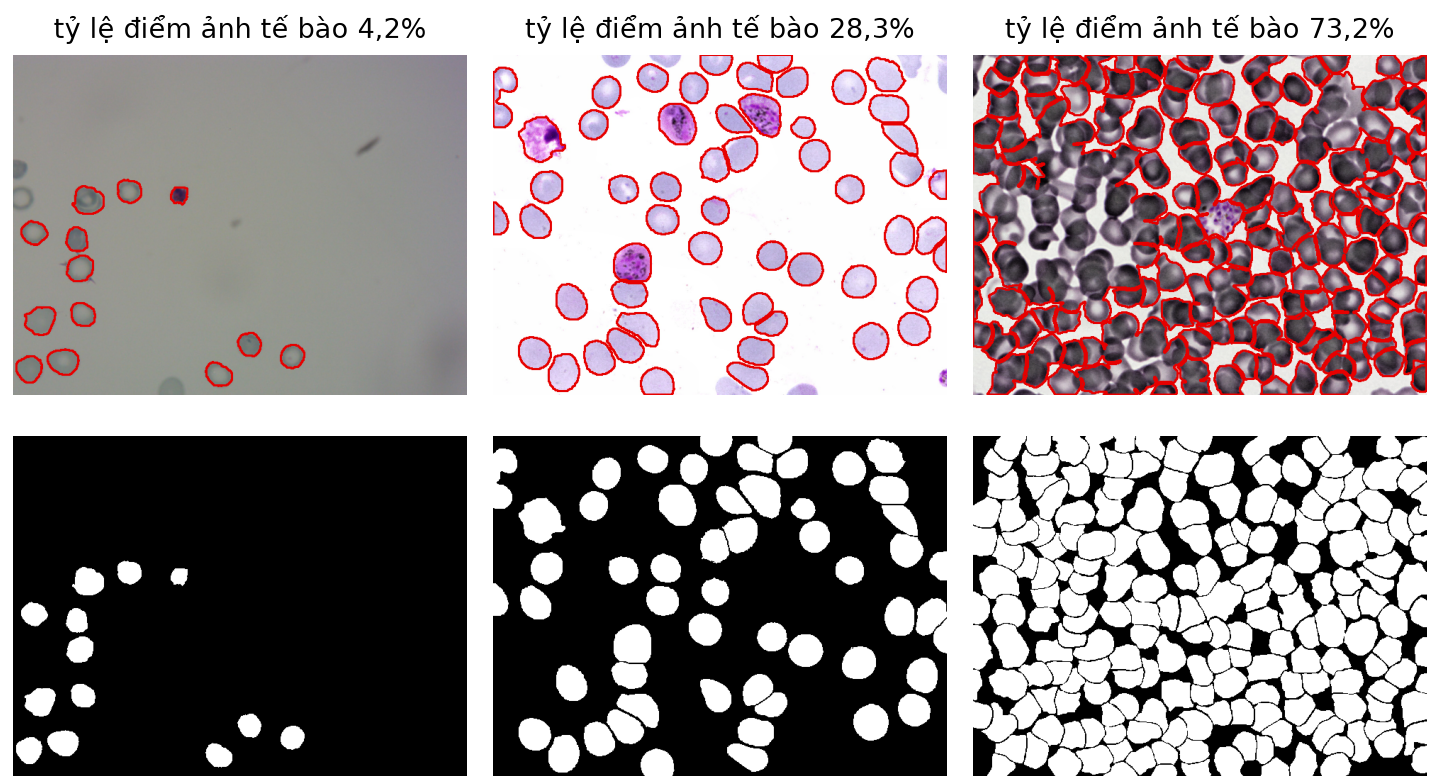
\includegraphics[width=\textwidth]{dataset_examples.png}
  \caption{Ba ảnh trong bộ dữ liệu có tỷ lệ điểm ảnh tế bào thấp nhất, ở mức trung vị và cao nhất. Hàng trên: ảnh gốc với đường viền mặt nạ chuẩn (màu đỏ). Hàng dưới: mặt nạ nhị phân. Ảnh đã được thu nhỏ về $640\times480$.}
  \label{fig:dataset}
\end{figure}

Hình~\ref{fig:dataset} cho phép rút ra ba quan sát. Một là, ba ảnh có nền và tông màu rất khác nhau, phù hợp với nhận định về độ biến thiên màu ở Chương~\ref{chap:tongquan}. Hai là, những tế bào có vùng bắt màu tím đậm ở ảnh giữa được gán cùng lớp với các tế bào còn lại, nên mặt nạ không phân biệt loại tế bào. Ba là, ở ảnh có mật độ cao, các tế bào chạm nhau được tách bằng các đường nền rất mảnh. Khi ảnh được thu nhỏ về $224\times224$ để đưa vào mạng, nhiều đường tách này bị mất. Vì vậy, sai số có xu hướng tập trung ở vùng tiếp giáp giữa các tế bào.

\subsection{Tiền xử lý và phân chia dữ liệu}

Ảnh được thu nhỏ một lần về $640\times480$, dùng nội suy theo diện tích cho ảnh và nội suy láng giềng gần nhất cho mặt nạ. Mặt nạ sau đó được nhị phân hóa với ngưỡng 127. Dữ liệu được xáo trộn với hạt giống cố định 2026 rồi chia theo tỷ lệ 70/10/20 thành tập huấn luyện, kiểm định và kiểm thử (Bảng~\ref{tab:split}). Các tập con có nhãn được lấy từ đầu danh sách huấn luyện đã xáo trộn, nên tập 5\% nằm trọn trong tập 10\%, và tập 10\% nằm trọn trong tập 20\%. Phần còn lại của tập huấn luyện được dùng như ảnh không nhãn: mặt nạ của chúng có trên đĩa nhưng không bao giờ được đọc khi huấn luyện. Khi đưa vào mạng, ảnh được thu nhỏ tiếp về $224\times224$, không giữ tỷ lệ khung hình $4:3$, và chuẩn hóa theo thống kê của ImageNet do Swin-Unet được tiền huấn luyện trên ImageNet~\cite{deng2009imagenet}.

\begin{table}[ht]
\centering
\caption{Phân chia dữ liệu. Tập kiểm định và kiểm thử giống nhau ở mọi tỷ lệ nhãn.}
\label{tab:split}
\small
\begin{tabular}{lcccc}
\toprule
Tập & Số ảnh & 5\% nhãn & 10\% nhãn & 20\% nhãn \\
\midrule
Huấn luyện (có nhãn / không nhãn) & 930 & 46 / 884 & 93 / 837 & 186 / 744 \\
Kiểm định                          & 133 & \multicolumn{3}{c}{133} \\
Kiểm thử                           & 265 & \multicolumn{3}{c}{265} \\
\midrule
Tổng                               & 1\,328 & & & \\
\bottomrule
\end{tabular}
\end{table}

\subsection{Tăng cường dữ liệu}

Tăng cường dữ liệu được thực hiện trực tuyến và chỉ áp dụng cho ảnh có nhãn. Ảnh không nhãn, ảnh kiểm định và ảnh kiểm thử chỉ được thu nhỏ và chuẩn hóa. Bảng~\ref{tab:aug} liệt kê các phép biến đổi. Nhóm hình học áp dụng đồng thời lên ảnh và mặt nạ, còn nhóm màu và chất lượng ảnh chỉ áp dụng lên ảnh. Phép biến thiên nhuộm trong không gian HED~\cite{tellez2018hed} vốn được thiết kế cho ảnh mô bệnh học nhuộm H\&E. Đề tài dùng nó như một xấp xỉ cho sự thay đổi cường độ thuốc nhuộm giữa các tiêu bản máu, với biên độ nhỏ để tránh làm bạc màu nền.

\begin{table}[ht]
\centering
\caption{Các phép tăng cường dữ liệu cho ảnh có nhãn ($p$: xác suất áp dụng).}
\label{tab:aug}
\small
\begin{tabularx}{\textwidth}{>{\raggedright\arraybackslash}p{2.6cm} >{\raggedright\arraybackslash}p{4.4cm} >{\raggedright\arraybackslash}X}
\toprule
Nhóm & Phép biến đổi & Tham số \\
\midrule
Hình học & Lật ngang, lật dọc, xoay $90^\circ$ & $p=0{,}5$ mỗi phép \\
         & Biến đổi affine & $p=0{,}5$; tỷ lệ $0{,}85$--$1{,}15$; xoay $\pm15^\circ$; dịch $\pm5\%$ \\
         & Biến dạng đàn hồi & $p=0{,}2$; $\alpha=30$, $\sigma=6$ \\
Màu và nhuộm & Color jitter & $p=0{,}5$; độ sáng, tương phản, bão hòa $\pm20\%$; sắc độ $\pm0{,}05$ \\
             & Biến thiên nhuộm HED & $p=0{,}5$; hệ số nhân $U(0{,}95;1{,}05)$; độ dịch $U(-0{,}005;0{,}005)$ \\
             & Gamma; CLAHE & $p=0{,}2$, $\gamma\in[0{,}8;1{,}2]$; $p=0{,}1$ \\
Chất lượng ảnh & Làm mờ Gauss; nhiễu Gauss & $p=0{,}1$, nhân $3$--$5$; $p=0{,}1$, độ lệch chuẩn $0{,}01$--$0{,}04$ \\
\bottomrule
\end{tabularx}
\end{table}

\subsection{Huấn luyện và thu nhận kết quả}

Mọi mô hình được huấn luyện 30\,000 vòng lặp bằng SGD với tốc độ học ban đầu 0,01, momentum 0,9 và weight decay $10^{-4}$. Tốc độ học giảm theo đa thức $\mathrm{lr}_t=0{,}01\,(1-t/30\,000)^{0{,}9}$~\cite{chen2018deeplab}. Huấn luyện dùng độ chính xác hỗn hợp FP16~\cite{micikevicius2018amp} trên GPU của nền tảng Kaggle. Mô hình học có giám sát dùng lô 8 ảnh có nhãn. Các phương pháp bán giám sát dùng lô gồm 1 ảnh có nhãn và 4 ảnh không nhãn, ghép thành một lần lan truyền xuôi. Cứ sau 500 vòng lặp, mô hình UNeXt được đánh giá bằng DSC trung bình trên tập kiểm định. Trọng số cho DSC kiểm định cao nhất được giữ lại và chỉ được đánh giá một lần trên tập kiểm thử. Mỗi cấu hình được huấn luyện một lần với hạt giống 2026.

Mỗi lần huấn luyện tạo ra ba loại dữ liệu phục vụ ba câu hỏi nghiên cứu. Bốn độ đo trên từng ảnh kiểm thử là dữ liệu chính cho CH1. Trọng số mô hình tốt nhất cho phép tính lại dự đoán trên từng ảnh, từ đó tính các đại lượng về loại lỗi cho CH2. Log huấn luyện ghi giá trị từng số hạng mất mát sau mỗi 100 vòng và DSC kiểm định sau mỗi 500 vòng, là dữ liệu cho CH3.

\section{Phân tích dữ liệu}

\subsection{Tính các độ đo}

Dự đoán được lấy theo lớp có xác suất lớn nhất và so sánh với mặt nạ ở độ phân giải $224\times224$. Biên của mặt nạ là tập điểm ảnh bị loại bỏ khi co mặt nạ bằng phần tử cấu trúc chữ thập $3\times3$. HD95 và ASD được tính theo đơn vị điểm ảnh ở độ phân giải này. Chúng không quy đổi được sang đơn vị vật lý, vì bộ dữ liệu không cung cấp kích thước thực của điểm ảnh. Kết quả được báo cáo dưới dạng trung bình (độ lệch chuẩn) trên 265 ảnh kiểm thử.

\subsection{Kiểm định thống kê (CH1)}

Vì mỗi phương pháp chỉ được huấn luyện một lần, khác biệt giữa DACL và từng mô hình khác được kiểm định bằng phép kiểm định hạng có dấu Wilcoxon~\cite{wilcoxon1945} trên cặp DSC của từng ảnh kiểm thử. Phép kiểm định này không giả định phân phối chuẩn, phù hợp với phân phối lệch của điểm số theo ảnh. Do DACL được so sánh với mười mô hình, ngưỡng ý nghĩa được hiệu chỉnh theo Bonferroni~\cite{dunn1961} thành $0{,}05/10=0{,}005$. Cách làm tương tự được áp dụng cho HD95 khi phân tích độ chính xác biên. Phép kiểm định này chỉ phản ánh sự biến thiên giữa các ảnh. Nó không tính đến dao động khi huấn luyện lại với hạt giống khác.

\subsection{Phân tích loại lỗi và độ khó của ảnh (CH2)}
\label{sec:analysis-rq2}

Để biết lợi ích của DACL đến từ loại lỗi nào, tất cả mô hình được chạy lại trên tập kiểm thử. Từ đó, đề tài tính độ chính xác (precision), độ phủ (recall) và tỷ lệ giữa diện tích dự đoán với diện tích mặt nạ chuẩn trên từng ảnh. Để biết lợi ích tập trung ở những ảnh nào, các ảnh kiểm thử được chia thành bốn nhóm theo tứ phân vị DSC của UNeXt học có giám sát, rồi so sánh hiệu DSC trong từng nhóm. Phần định tính dùng bốn ảnh có độ lệch chuẩn DSC giữa các mô hình lớn nhất. Tiêu chí khách quan này tránh việc chọn ảnh có lợi cho một phương pháp cụ thể.

\subsection{Phân tích diễn biến huấn luyện (CH3)}

Bên cạnh phân tích lý thuyết ở mục~\ref{sec:loss-analysis} và~\ref{sec:weights}, độ ổn định của DACL được đánh giá qua đường DSC kiểm định theo vòng lặp. Đường của DACL được so sánh với UNeXt học có giám sát và với hai phương pháp đối chứng tiêu biểu. Độ ổn định ở giai đoạn cuối được đo bằng trung bình và độ lệch chuẩn của DSC kiểm định trong 10\,000 vòng cuối.

Chương này đã mô tả khung nghiên cứu, gồm cách xây dựng mô hình DACL, phân tích các thành phần mất mát và căn cứ lựa chọn trọng số, cùng cách thu thập và phân tích dữ liệu cho từng câu hỏi nghiên cứu. Chương~\ref{chap:ketqua} trình bày các kết quả thu được, còn Chương~\ref{chap:ketluan} tóm tắt, rút ra kết luận và thảo luận ý nghĩa của chúng.

% =====================================================================
\chapter{Kết quả nghiên cứu}
\label{chap:ketqua}

Chương này trình bày kết quả theo thứ tự của ba câu hỏi nghiên cứu. Mục~\ref{sec:res-fs} báo cáo kết quả học có giám sát, làm bối cảnh để đọc các kết quả còn lại. Mục~\ref{sec:res-rq1} trả lời CH1 bằng cách so sánh DACL với tám phương pháp bán giám sát và với học có giám sát. Mục~\ref{sec:res-rq2} và~\ref{sec:res-qual} trả lời CH2, lần lượt bằng phân tích định lượng về loại lỗi và độ khó của ảnh, và bằng quan sát định tính. Mục~\ref{sec:res-dynamics} trình bày diễn biến huấn luyện của DACL, bổ sung bằng chứng thực nghiệm cho CH3. Người đọc chỉ cần các kết luận có thể chuyển thẳng sang Chương~\ref{chap:ketluan}. Mọi con số trong chương được tính từ các tệp kết quả lưu trong thư mục \texttt{results/} của kho mã nguồn.

\section{Kết quả học có giám sát}
\label{sec:res-fs}

Bảng~\ref{tab:fs} cho thấy khi số ảnh có nhãn tăng từ 5\% (46 ảnh) lên 100\% (930 ảnh), DSC của UNeXt chỉ tăng từ 94,15\% lên 95,23\%, tức là 1,08 điểm. Với Swin-Unet, mức tăng là 0,73 điểm. Như vậy, trên bộ dữ liệu này và ở độ phân giải $224\times224$, chỉ 46 ảnh có nhãn đã đủ để đạt phần lớn độ chính xác có thể đạt được. Dư địa mà học bán giám sát có thể cải thiện so với học có giám sát trên cùng số nhãn chỉ khoảng một điểm DSC.

\begin{table}[ht]
\centering
\caption{Kết quả học có giám sát trên tập kiểm thử theo tỷ lệ ảnh có nhãn. DSC và Jaccard tính bằng \%, HD95 và ASD tính bằng điểm ảnh ở độ phân giải $224\times224$.}
\label{tab:fs}
\small
\begin{tabular}{llcccc}
\toprule
Mạng & Nhãn & DSC $\uparrow$ & Jaccard $\uparrow$ & HD95 $\downarrow$ & ASD $\downarrow$ \\
\midrule
\inputtable{tables/fs.tex}
\bottomrule
\end{tabular}
\end{table}

Swin-Unet cao hơn UNeXt ở mọi mức nhãn, từ 0,10 đến 0,57 điểm DSC, và khoảng cách lớn nhất ở mức 5\% nhãn. Đây là khoảng cách mà DACL hướng tới thu hẹp: đưa UNeXt đến gần độ chính xác của Swin-Unet, trong khi chi phí suy luận chỉ bằng khoảng một phần bảy (Bảng~\ref{tab:complexity}).

\section{Độ chính xác của DACL so với các phương pháp khác (CH1)}
\label{sec:res-rq1}

Bảng~\ref{tab:ssl5} và~\ref{tab:ssl10} trình bày kết quả của mười một mô hình ở mức 5\% và 10\% nhãn. Cột $p$ là kết quả kiểm định Wilcoxon theo cặp trên DSC của từng ảnh, so với DACL.

\begin{table}[p]
\centering
\caption{Kết quả trên tập kiểm thử với 5\% ảnh có nhãn. DSC và Jaccard tính bằng \%, HD95 và ASD tính bằng điểm ảnh ở độ phân giải $224\times224$. Trong nhóm bán giám sát, giá trị tốt nhất được \textbf{in đậm} và tốt thứ hai được \textit{in nghiêng}. Cột $p$: kiểm định Wilcoxon theo cặp trên DSC của từng ảnh so với DACL; ngưỡng ý nghĩa sau hiệu chỉnh Bonferroni là 0,005.}
\label{tab:ssl5}
\resizebox{\textwidth}{!}{%
\begin{tabular}{lcccccccc}
\toprule
Phương pháp & Có nhãn & Không nhãn & DSC $\uparrow$ & Jaccard $\uparrow$ & HD95 $\downarrow$ & ASD $\downarrow$ & $p$ \\
\midrule
\inputtable{tables/ssl_5.tex}
\bottomrule
\end{tabular}}
\end{table}

\begin{table}[p]
\centering
\caption{Kết quả trên tập kiểm thử với 10\% ảnh có nhãn. Quy ước như Bảng~\ref{tab:ssl5}.}
\label{tab:ssl10}
\resizebox{\textwidth}{!}{%
\begin{tabular}{lcccccccc}
\toprule
Phương pháp & Có nhãn & Không nhãn & DSC $\uparrow$ & Jaccard $\uparrow$ & HD95 $\downarrow$ & ASD $\downarrow$ & $p$ \\
\midrule
\inputtable{tables/ssl_10.tex}
\bottomrule
\end{tabular}}
\end{table}

\subsection{Độ trùng khớp}

Ở cả hai mức nhãn, DACL có DSC và Jaccard cao nhất trong nhóm bán giám sát. Ở mức 5\%, DACL đạt DSC 94,38\%, hơn phương pháp đứng thứ hai là PCPCS 0,39 điểm và hơn MT 1,21 điểm. Ở mức 10\%, DACL đạt 94,46\%, hơn DSTCT, phương pháp đứng thứ hai, 0,60 điểm. Khác biệt giữa DACL và từng phương pháp bán giám sát đều có ý nghĩa thống kê sau hiệu chỉnh Bonferroni ($p<0{,}001$). Xét riêng nhóm CNN--Transformer, DACL hơn LMCT 0,64 điểm ở mức 5\% và 0,92 điểm ở mức 10\%.

So với học có giám sát trên cùng số ảnh có nhãn, kết quả khác đi. Ở mức 5\%, DACL cao hơn UNeXt học có giám sát 0,23 điểm, nhưng khác biệt không có ý nghĩa thống kê ($p=0{,}073$). Ở mức 10\%, DACL thấp hơn 0,14 điểm, và khác biệt có ý nghĩa ($p<0{,}001$). Tám phương pháp đối chứng đều thấp hơn UNeXt học có giám sát ở cả hai mức. DACL là phương pháp bán giám sát duy nhất không thua kém có ý nghĩa ở mức 5\%. Swin-Unet học có giám sát cao hơn DACL 0,34 điểm ở mức 5\% và 0,55 điểm ở mức 10\%.

\subsection{Độ chính xác biên}

Về biên, DACL không giữ được vị trí dẫn đầu. HD95 của DACL ở mức 5\% là 3,01 điểm ảnh, đứng thứ tám trong chín phương pháp bán giám sát, chỉ trên DSTCT. Kiểm định Wilcoxon với hiệu chỉnh Bonferroni cho thấy ICT, MT, DCT và CPS có HD95 thấp hơn DACL một cách có ý nghĩa, với mức chênh 0,12--0,20 điểm ảnh. Ở mức 10\%, HD95 của DACL (2,97) đứng thứ sáu, và MT, PCPCS, DCT, CTCT thấp hơn có ý nghĩa. Ngược lại, ASD của DACL thuộc nhóm tốt nhất: thứ hai ở mức 5\% (0,81, sau CPS với 0,80) và tốt nhất ở mức 10\% (0,80). Hai độ đo biên cho kết quả khác nhau vì ASD là trung bình khoảng cách trên mọi điểm biên, còn HD95 bị chi phối bởi 5\% điểm biên xa nhất. Kết quả này gợi ý rằng DACL khớp biên tốt ở phần lớn tế bào, nhưng sinh ra một số vùng sai lệch nằm xa tế bào thật. Các mức chênh 0,1--0,2 điểm ảnh ở độ phân giải $224\times224$ đều rất nhỏ so với kích thước một tế bào.

\subsection{Ảnh hưởng của số lượng nhãn}

Khi tăng từ 5\% lên 10\% nhãn, DSC của DACL tăng 0,08 điểm, còn của UNeXt học có giám sát tăng 0,45 điểm. Một số phương pháp đối chứng lại giảm: CPS giảm 0,87, PCPCS giảm 0,36, DCT giảm 0,35 và LMCT giảm 0,20 điểm. Nhân đôi số ảnh có nhãn về lý thuyết không nên làm mô hình kém đi. Vì vậy, các mức giảm này nhiều khả năng phản ánh dao động giữa các lần huấn luyện, do mỗi cấu hình chỉ được chạy một lần. Biên độ của dao động, có trường hợp gần 0,9 điểm, cùng bậc với khoảng cách giữa các phương pháp đối chứng. Ngược lại, vị trí dẫn đầu của DACL được lặp lại ở cả hai mức nhãn, với khoảng cách 0,39--0,60 điểm so với phương pháp thứ hai.

\section{Loại lỗi và độ khó của ảnh (CH2): kết quả định lượng}
\label{sec:res-rq2}

\subsection{Độ chính xác và độ phủ}

Toàn bộ 22 mô hình được chạy lại trên tập kiểm thử. DSC tính lại khớp với kết quả lưu khi huấn luyện đến hai chữ số thập phân. Bảng~\ref{tab:precrec} trình bày precision, recall và tỷ lệ diện tích dự đoán so với mặt nạ chuẩn.

\begin{table}[ht]
\centering
\caption{Độ chính xác, độ phủ (\%) và tỷ lệ diện tích dự đoán so với mặt nạ chuẩn, lấy trung bình trên 265 ảnh kiểm thử.}
\label{tab:precrec}
\small
\begin{tabular}{lcccccc}
\toprule
 & \multicolumn{3}{c}{5\% nhãn} & \multicolumn{3}{c}{10\% nhãn} \\
\cmidrule(lr){2-4}\cmidrule(lr){5-7}
Phương pháp & Precision & Recall & Diện tích & Precision & Recall & Diện tích \\
\midrule
\inputtable{tables/precrec.tex}
\bottomrule
\end{tabular}
\end{table}

Bảng~\ref{tab:precrec} cho ba kết quả. Thứ nhất, mọi mô hình, kể cả hai mô hình học có giám sát, đều dự đoán diện tích lớn hơn mặt nạ chuẩn từ 2\% đến 6\%. Thứ hai, tất cả các phương pháp bán giám sát đều có precision thấp hơn UNeXt học có giám sát, tức là sinh ra nhiều dương tính giả hơn. Thứ ba, DACL có precision cao nhất trong nhóm bán giám sát ở cả hai mức nhãn. Recall của DACL cũng cao nhất ở mức 5\%, và chỉ thấp hơn LMCT ở mức 10\%. LMCT đạt recall cao nhờ dự đoán lấn biên nhiều nhất: diện tích lớn hơn mặt nạ chuẩn 6\%, kéo theo precision thấp nhất. Ưu thế DSC của DACL vì vậy đến từ việc giảm đồng thời cả hai loại lỗi so với các phương pháp bán giám sát khác, chứ không phải từ việc đánh đổi loại lỗi này lấy loại lỗi kia.

\subsection{Phân bố lợi ích theo độ khó của ảnh}

Ở mức 5\% nhãn, DSC trung bình của DACL cao hơn UNeXt học có giám sát, nhưng DACL chỉ tốt hơn trên 98 trong 265 ảnh. Trung vị của hiệu DSC giữa hai mô hình là $-0{,}12$ điểm. Bảng~\ref{tab:quartile} chia ảnh kiểm thử thành bốn nhóm theo tứ phân vị DSC của UNeXt học có giám sát, từ nhóm khó nhất (Q1) đến nhóm dễ nhất (Q4).

\begin{table}[ht]
\centering
\caption{Hiệu DSC trung bình (điểm \%) so với UNeXt học có giám sát, theo nhóm tứ phân vị độ khó. Mỗi nhóm có 66 hoặc 67 ảnh.}
\label{tab:quartile}
\small
\begin{tabular}{lccc ccc}
\toprule
 & \multicolumn{3}{c}{5\% nhãn} & \multicolumn{3}{c}{10\% nhãn} \\
\cmidrule(lr){2-4}\cmidrule(lr){5-7}
Nhóm & DACL & CPS & FS Swin-Unet & DACL & CPS & FS Swin-Unet \\
\midrule
Q1 (khó nhất) & $+1{,}42$ & $+0{,}31$ & $+1{,}31$ & $+0{,}34$ & $-1{,}03$ & $+0{,}90$ \\
Q2            & $-0{,}01$ & $-0{,}25$ & $+0{,}35$ & $-0{,}12$ & $-1{,}30$ & $+0{,}29$ \\
Q3            & $-0{,}16$ & $-0{,}36$ & $+0{,}41$ & $-0{,}27$ & $-1{,}64$ & $+0{,}29$ \\
Q4 (dễ nhất)  & $-0{,}31$ & $-0{,}39$ & $+0{,}21$ & $-0{,}48$ & $-1{,}96$ & $+0{,}17$ \\
\bottomrule
\end{tabular}
\end{table}

Ở mức 5\%, DACL cải thiện trung bình 1,42 điểm trên nhóm khó nhất. Riêng 20 ảnh mà UNeXt học có giám sát đạt DSC dưới 90\%, mức cải thiện là 3,75 điểm. Ngược lại, DACL kém hơn một chút trên ba nhóm còn lại, và mức kém lớn nhất ($-0{,}31$) rơi vào nhóm dễ nhất. Mức 10\% có cùng xu hướng nhưng yếu hơn: $+0{,}34$ ở Q1 và $-0{,}48$ ở Q4. Vì các nhóm được xác định theo chính điểm số của UNeXt học có giám sát, nhóm Q1 chứa cả những ảnh mà mô hình này kém do ngẫu nhiên. Bất kỳ mô hình nào khác cũng có xu hướng tốt hơn ở nhóm đó, theo hiện tượng hồi quy về trung bình. Cột Swin-Unet học có giám sát phản ánh rõ hiệu ứng này. Điểm phân biệt DACL nằm ở hai đầu bảng. Ở Q1, mức cải thiện của DACL tương đương Swin-Unet học có giám sát, một mạng lớn gấp 17 lần. Ở Q4, DACL lại kém UNeXt học có giám sát, trong khi Swin-Unet vẫn tốt hơn. CPS, chỉ giám sát chéo giữa hai mạng UNeXt mà không có Swin-Unet và $\Ldac$, có mức cải thiện ở Q1 thấp hơn nhiều.

\section{Loại lỗi và độ khó của ảnh (CH2): kết quả định tính}
\label{sec:res-qual}

Hình~\ref{fig:qual} so sánh dự đoán của UNeXt học có giám sát và năm phương pháp bán giám sát gần đây nhất ở mức 5\% nhãn, trên bốn ảnh kiểm thử được chọn theo tiêu chí ở mục~\ref{sec:analysis-rq2}.

\begin{figure}[ht]
  \centering
  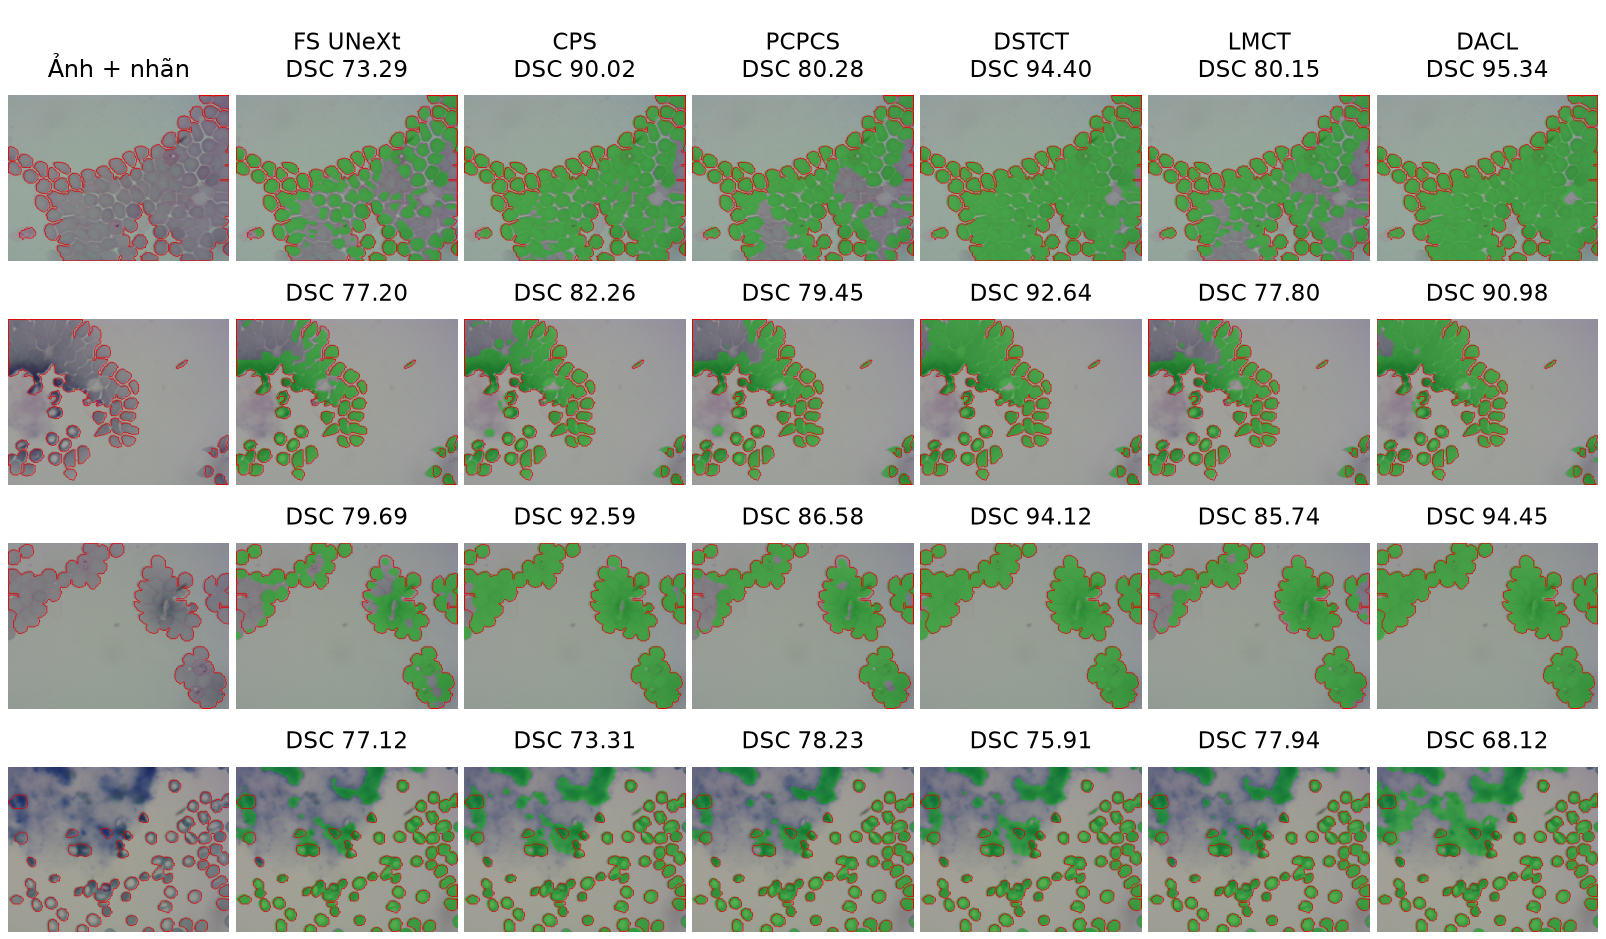
\includegraphics[width=\textwidth]{qualitative_5p.png}
  \caption{Kết quả phân đoạn trên bốn ảnh kiểm thử ở mức 5\% nhãn. Vùng tô xanh: dự đoán. Đường viền đỏ: mặt nạ chuẩn. Số trên mỗi ô là DSC (\%) của ảnh đó. Ảnh được chọn là bốn ảnh có độ lệch chuẩn DSC giữa các mô hình lớn nhất.}
  \label{fig:qual}
\end{figure}

Ba ảnh đầu có chung đặc điểm: tế bào xếp thành cụm dày đặc hoặc chạm nhau thành mảng lớn. UNeXt học có giám sát bỏ sót phần lớn bên trong các cụm này (DSC 73--80\%). DACL và DSTCT, hai phương pháp có giáo viên EMA của Swin-Unet, phủ gần trọn các cụm và đạt DSC trên 90\%. CPS cũng cải thiện đáng kể, còn PCPCS và LMCT cải thiện ít hơn. Ảnh thứ tư cho thấy trường hợp ngược lại. Góc trên bên trái của ảnh có một mảng bắt màu xanh đậm không phải tế bào, và mọi mô hình đều dự đoán nhầm một phần mảng này. DACL nhầm nhiều nhất, với DSC 68,12\%, thấp nhất trong sáu mô hình. Trường hợp này phù hợp với HD95 kém của DACL ở mục~\ref{sec:res-rq1}. Tuy nhiên, nó không đại diện cho toàn bộ tập kiểm thử, vì precision trung bình của DACL vẫn cao nhất trong nhóm bán giám sát. Bốn ảnh không đủ để khái quát, nên hình này chỉ minh họa cho các xu hướng đã đo bằng số liệu ở mục trước.

\section{Diễn biến huấn luyện của DACL (CH3)}
\label{sec:res-dynamics}

Hình~\ref{fig:curves} trình bày DSC kiểm định của UNeXt theo vòng lặp với DACL, hai phương pháp đối chứng CPS và DSTCT, và UNeXt học có giám sát.

\begin{figure}[ht]
  \centering
  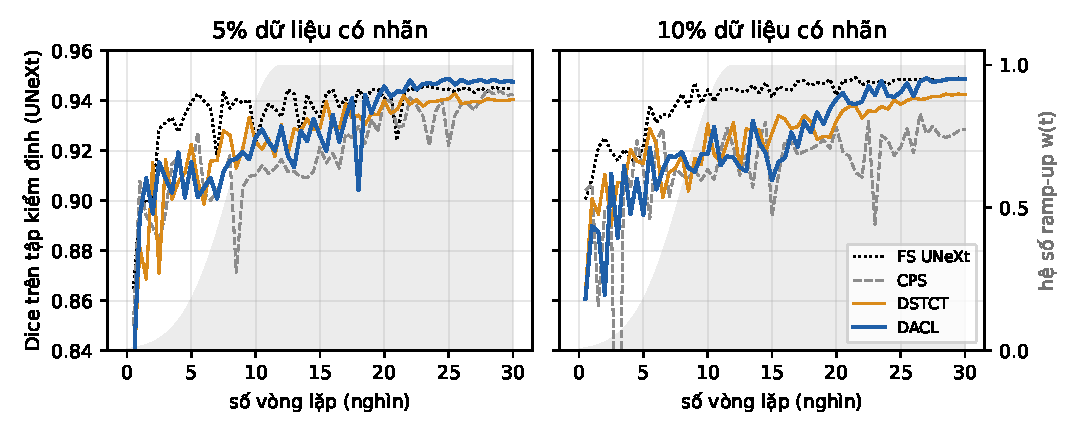
\includegraphics[width=\textwidth]{val_curves.pdf}
  \caption{DSC trên tập kiểm định của UNeXt theo vòng lặp, đo mỗi 500 vòng. Vùng tô xám là hệ số ramp-up $w(t)$ của các phương pháp bán giám sát (trục phải). Trục tung bị cắt ở 0,84.}
  \label{fig:curves}
\end{figure}

Với bộ trọng số $\{0{,}2;\,0{,}2;\,1\}$, DACL huấn luyện ổn định ở cả hai mức nhãn. DSC kiểm định cao nhất đạt 0,9489 ở vòng 25\,000 với 5\% nhãn và 0,9490 ở vòng 27\,000 với 10\% nhãn, đều trong giai đoạn cuối khi tốc độ học đã giảm. Trong 10\,000 vòng cuối, DSC kiểm định của DACL ở mức 5\% có trung bình 0,9467 và độ lệch chuẩn 0,0019. Các giá trị tương ứng của CPS là 0,9370 và 0,0063, của DSTCT là 0,9396 và 0,0017, và của UNeXt học có giám sát là 0,9434 và 0,0045. Ở mức 10\%, DACL đạt 0,9447 với độ lệch chuẩn 0,0036, cao hơn CPS (0,9225; 0,0095) và DSTCT (0,9389; 0,0031) nhưng thấp hơn UNeXt học có giám sát (0,9479; 0,0015). Thứ tự này khớp với kết quả trên tập kiểm thử ở mục~\ref{sec:res-rq1}.

Sau khi hệ số ramp-up đạt giá trị đầy đủ, đường DSC kiểm định của DACL chỉ có hai lần giảm tạm thời: xuống 0,904 ở vòng 18\,000 với 5\% nhãn, và xuống 0,908 ở vòng 15\,000 với 10\% nhãn. Cả hai đều hồi phục ngay ở lần đánh giá kế tiếp, lên 0,942 và 0,915. Log huấn luyện cho thấy, sau vòng 12\,000, phần không giám sát sau khi nhân trọng số chỉ bằng trung bình 18\% phần có giám sát, và không vượt quá 27\% ở cả hai mức nhãn. Như vậy, trong suốt quá trình huấn luyện, tín hiệu giám sát thật vẫn giữ vai trò chủ đạo, đúng như mục tiêu khi lựa chọn trọng số ở mục~\ref{sec:weights}. Hình~\ref{fig:curves} cũng cho thấy UNeXt học có giám sát tăng nhanh hơn hẳn các phương pháp bán giám sát trong 8\,000 vòng đầu, điều sẽ được thảo luận ở Chương~\ref{chap:ketluan}.

\section{Tóm tắt chương}

Chương~\ref{chap:ketqua} đã trình bày kết quả định lượng và định tính cho ba câu hỏi nghiên cứu. Với CH1, DACL có độ trùng khớp cao nhất trong nhóm bán giám sát ở cả hai mức nhãn, nhưng không vượt rõ học có giám sát trên cùng số nhãn và không dẫn đầu về HD95. Với CH2, lợi ích của DACL đến từ việc giảm đồng thời dương tính giả và âm tính giả, và tập trung ở nhóm ảnh khó nhất, đặc biệt là các cụm tế bào dày đặc. Với CH3, DACL huấn luyện ổn định với bộ trọng số đã chọn, và tín hiệu giám sát giữ vai trò chủ đạo trong suốt quá trình huấn luyện. Chương~\ref{chap:ketluan} tóm tắt toàn bộ nghiên cứu, rút ra kết luận cho từng câu hỏi, thảo luận các kết quả trong mối liên hệ với nghiên cứu trước và đưa ra khuyến nghị.

% =====================================================================
\chapter{Tóm tắt, kết luận, thảo luận và khuyến nghị}
\label{chap:ketluan}

Chương này tổng kết toàn bộ nghiên cứu. Mục~\ref{sec:summary} tóm tắt mục đích, câu hỏi, tổng quan, phương pháp và kết quả. Mục~\ref{sec:conclusion} rút ra kết luận cho từng câu hỏi nghiên cứu. Mục~\ref{sec:discussion} thảo luận các kết luận trong mối liên hệ với cơ sở lý thuyết và các nghiên cứu liên quan, đồng thời nêu giới hạn của đề tài. Hai mục tiếp theo đưa ra khuyến nghị cho thực tiễn và gợi ý cho nghiên cứu tiếp theo. Mục cuối là kết luận chung.

\section{Tóm tắt}
\label{sec:summary}

Đề tài xây dựng một mô hình phân đoạn tế bào máu trong ảnh hiển vi dựa trên khung học bán giám sát DACL~\cite{wang2026dacl}, nhằm giảm nhu cầu về mặt nạ gán nhãn. Ba câu hỏi được đặt ra: DACL chính xác đến đâu so với các phương pháp bán giám sát khác và so với học có giám sát (CH1); lợi ích của DACL nằm ở loại lỗi nào và ở những ảnh nào (CH2); các thành phần mất mát của DACL tương tác ra sao, và cần chọn trọng số thế nào để huấn luyện ổn định (CH3).

Tổng quan tài liệu cho thấy ảnh tế bào máu có nhiều đối tượng nhỏ, ranh giới mảnh giữa các tế bào chạm nhau và màu nhuộm biến thiên mạnh. Các phương pháp bán giám sát hiện có đều phải cân bằng giữa việc khai thác nhãn giả và nguy cơ thiên lệch xác nhận. DACL kết hợp giám sát giả chéo giữa UNeXt và Swin-Unet, nhất quán nội suy với giáo viên EMA, và một hàm mất mát đồng thuận kép trên toàn bộ phân phối xác suất của hai mạng.

Về phương pháp, đề tài dùng thiết kế thực nghiệm có đối chứng. DACL và tám phương pháp bán giám sát được xây dựng lại từ đầu trong cùng một khung mã. Tất cả được huấn luyện trên bộ dữ liệu Blood Cell Segmentation gồm 1\,328 ảnh, với cùng cách chia dữ liệu và chế độ huấn luyện, ở hai mức 5\% và 10\% nhãn. Đề tài phân tích số hạng entropy của hàm mất mát đồng thuận kép và độ lớn của các thành phần mất mát, từ đó chọn bộ trọng số $\{0{,}2;\,0{,}2;\,1\}$. Kết quả được đánh giá bằng DSC, Jaccard, HD95, ASD, kiểm định Wilcoxon theo cặp, phân tích precision và recall, và phân tích theo nhóm độ khó.

Kết quả cho thấy DACL đạt DSC 94,38\% ở mức 5\% và 94,46\% ở mức 10\% nhãn, cao nhất trong nhóm bán giám sát với khác biệt có ý nghĩa thống kê. DACL có precision cao nhất trong nhóm, và cải thiện 1,42 điểm DSC so với UNeXt học có giám sát trên nhóm ảnh khó nhất. Tuy nhiên, DACL không vượt rõ UNeXt học có giám sát trên cùng số nhãn, và có HD95 kém hơn một số phương pháp đơn giản. Quá trình huấn luyện ổn định, với phần không giám sát chỉ bằng khoảng 18\% phần có giám sát sau giai đoạn ramp-up.

\section{Kết luận}
\label{sec:conclusion}

\textbf{Đối với CH1.} Trên ảnh hiển vi tế bào máu, DACL vượt cả tám phương pháp bán giám sát tiêu biểu về độ trùng khớp ở cả hai mức nhãn. Khoảng cách đến phương pháp đứng thứ hai là 0,39 điểm DSC ở mức 5\% và 0,60 điểm ở mức 10\%, đều có ý nghĩa thống kê. Kết luận này không mở rộng sang độ chính xác biên, vì HD95 của DACL chỉ ở mức trung bình đến kém trong nhóm. Nó cũng không mở rộng sang so sánh với học có giám sát: ở mức 5\%, DACL tương đương UNeXt học có giám sát, và ở mức 10\%, DACL thấp hơn một chút.

\textbf{Đối với CH2.} Lợi ích của DACL không đến từ việc đánh đổi loại lỗi này lấy loại lỗi kia. DACL giảm đồng thời dương tính giả và âm tính giả so với các phương pháp bán giám sát khác. Lợi ích tập trung ở nhóm ảnh khó nhất, chủ yếu là ảnh có cụm tế bào dày đặc mà UNeXt học có giám sát bỏ sót phần bên trong. Trên nhóm ảnh này, DACL cải thiện tương đương Swin-Unet học có giám sát. Cái giá là một mức giảm nhỏ trên ảnh dễ, và một số dự đoán nhầm trên vùng cặn nhuộm.

\textbf{Đối với CH3.} Số hạng entropy của hàm mất mát đồng thuận kép chứa hai tác động ngược chiều. Khi hai mạng đã đồng thuận, số hạng này trở thành cực tiểu hóa entropy với hệ số $\beta$. Kết hợp với nhãn giả cứng của $\Lcps$, các thành phần không giám sát của DACL cùng đẩy hai mạng về dự đoán tự tin. Do đó, độ ổn định của DACL phụ thuộc vào tỷ lệ giữa phần không giám sát và tín hiệu giám sát thật. Khi mỗi vòng lặp chỉ có một ảnh có nhãn, bộ trọng số $\{0{,}2;\,0{,}2;\,1\}$ giúp DACL huấn luyện ổn định, với tín hiệu giám sát giữ vai trò chủ đạo.

\section{Thảo luận}
\label{sec:discussion}

\subsection{Ưu thế của DACL trong nhóm bán giám sát}

DACL dẫn đầu nhóm bán giám sát ở cả hai mức nhãn. Một chi tiết đáng chú ý là DSTCT, phương pháp duy nhất ngoài DACL có giáo viên EMA của Swin-Unet, đứng thứ hai ở mức 10\%. Trong hình định tính, DSTCT cũng phủ các cụm tế bào dày đặc tốt tương đương DACL. Điều này gợi ý rằng mục tiêu ổn định từ một Transformer được tiền huấn luyện là thành phần đóng góp quan trọng. Kết quả cũng ủng hộ lập luận của Luo và cộng sự rằng cặp mạng dị thể giúp giám sát chéo hiệu quả hơn, vì hai loại mạng mắc lỗi ở những vị trí khác nhau~\cite{luo2022ctct}. Tuy nhiên, đề tài chưa thực hiện thí nghiệm loại bỏ từng thành phần, nên chưa thể tách phần đóng góp riêng của $\Ldac$ so với giáo viên EMA và giám sát chéo.

\subsection{Vì sao DACL không vượt rõ học có giám sát}

Mục tiêu của học bán giám sát là dùng ảnh không nhãn để vượt mô hình chỉ học từ cùng số ảnh có nhãn. Trong đề tài, DACL chỉ đạt điều này ở mức tương đương. Có hai nguyên nhân.

Nguyên nhân thứ nhất là dư địa cải thiện hẹp. Trên bộ dữ liệu này, học có giám sát với 46 ảnh đã đạt 94,15\%, chỉ kém mức dùng toàn bộ 930 ảnh có nhãn 1,08 điểm. Khi phần lớn độ chính xác đã đạt được chỉ với ít nhãn, ảnh không nhãn có ít thông tin mới để bổ sung. Đóng góp của chúng khi đó dễ bị lấn át bởi nhiễu do nhãn giả mang lại, như mức giảm precision ở mọi phương pháp bán giám sát cho thấy.

Nguyên nhân thứ hai thuộc về thiết kế thí nghiệm. Mô hình học có giám sát dùng lô 8 ảnh có nhãn, còn các phương pháp bán giám sát dùng 1 ảnh có nhãn mỗi vòng. Qua 30\,000 vòng lặp, mô hình học có giám sát nhận 240\,000 lượt ảnh có nhãn, gấp tám lần các phương pháp bán giám sát, với gradient ít nhiễu hơn. Hình~\ref{fig:curves} phản ánh điều này: UNeXt học có giám sát tăng nhanh hơn hẳn trong giai đoạn đầu. So sánh giữa học có giám sát và học bán giám sát vì vậy có lợi cho học có giám sát. Trong khi đó, so sánh giữa các phương pháp bán giám sát với nhau không bị ảnh hưởng, vì chúng dùng chung một cách bố trí lô. Nhận định rằng ảnh không nhãn ít giá trị trên bộ dữ liệu này chỉ nên được đưa ra sau khi so sánh với học có giám sát dùng cùng cách bố trí lô.

\subsection{Độ chính xác biên}

Ràng buộc đồng thuận trên toàn bộ phân phối xác suất được kỳ vọng giúp đường biên chính xác hơn, nhưng HD95 của DACL không cho thấy điều đó. Có ba yếu tố có thể giải thích. Thứ nhất, trên ảnh tế bào máu, HD95 bị chi phối bởi một số ít vùng dương tính giả nằm xa tế bào thật, như mảng cặn nhuộm ở Hình~\ref{fig:qual}, chứ không phải bởi sai lệch nhỏ dọc đường viền. Thứ hai, theo phân tích ở mục~\ref{sec:loss-analysis}, $\Ldac$ có thành phần cực tiểu hóa entropy. Thành phần này làm dự đoán tự tin hơn, kể cả ở những vùng mà mô hình sai. Một dự đoán sai nhưng tự tin trên vùng cặn nhuộm sẽ tạo thành một vùng dương tính giả trọn vẹn thay vì rải rác. Đây là giả thuyết, chưa được kiểm chứng bằng thí nghiệm loại bỏ $\Lent$. Thứ ba, HD95 được tính ở $224\times224$, nơi các mức chênh 0,1--0,2 điểm ảnh giữa các phương pháp rất nhỏ so với kích thước tế bào. Vì vậy, khác biệt về HD95 tuy có ý nghĩa thống kê nhưng có ý nghĩa thực tiễn hạn chế.

\subsection{Lợi ích tập trung ở ảnh khó}

Kết quả ở CH2 phù hợp với ý tưởng thiết kế của DACL: chuyển tri thức từ Transformer dung lượng lớn sang CNN nhẹ~\cite{wang2026dacl}. Trên nhóm ảnh khó nhất, UNeXt huấn luyện bằng DACL cải thiện tương đương Swin-Unet học có giám sát. Hình định tính cho thấy đó chủ yếu là các cụm tế bào dày đặc, dạng ảnh ít xuất hiện trong 46 ảnh có nhãn. Ảnh không nhãn, thông qua Swin-Unet và giáo viên EMA, cung cấp thêm các ví dụ thuộc dạng này. Cần đọc kết quả với lưu ý về hồi quy về trung bình, vì các nhóm được xác định theo điểm số của chính UNeXt học có giám sát. Tuy vậy, sự khác biệt giữa DACL, CPS và Swin-Unet trong cùng một nhóm vẫn so sánh được. Mức giảm nhỏ của DACL trên ảnh dễ có thể là hệ quả của nhiễu từ nhãn giả trên những ảnh mà học có giám sát đã làm tốt. Về mặt ứng dụng, đây là sự đánh đổi có lợi, vì lỗi trên ảnh khó ảnh hưởng đến các phép đếm và đo phía sau nhiều hơn.

\subsection{Trọng số của các thành phần mất mát}

Phân tích ở CH3 cho thấy trọng số của DACL không phải là hằng số cố định của khung, mà phụ thuộc vào lượng tín hiệu giám sát trong mỗi vòng lặp. Với một ảnh có nhãn mỗi vòng, tăng trọng số lên mười lần khiến phần không giám sát lớn gấp nhiều lần phần có giám sát, và lần thử nghiệm sơ bộ với trọng số đó không ổn định. Điều này phù hợp với lý thuyết về thiên lệch xác nhận~\cite{arazo2020pseudo}: khi nhãn giả chi phối quá trình học, hai mạng có thể củng cố lỗi chung của nhau. Phân tích số hạng entropy bổ sung một góc nhìn. $\Lent$ tự nó không khuyến khích đồng thuận, mà khuyến khích sự tự tin. Do đó, $\beta$ cần được xem như hệ số của một số hạng cực tiểu hóa entropy, vốn được biết là có thể gây hại khi mô hình chưa đủ tốt~\cite{grandvalet2005entropy}.

Về tính công bằng, bộ trọng số của DACL do đề tài lựa chọn, trong khi các phương pháp đối chứng dùng giá trị theo công bố hoặc mã nguồn của từng phương pháp. Để hạn chế thiên lệch, bộ trọng số được xác định theo các căn cứ phân tích trước khi chạy thí nghiệm chính, và chỉ một cấu hình được dùng. Kết quả là trọng số của DACL nằm cùng bậc độ lớn với các phương pháp đối chứng. Tuy vậy, DACL vẫn là phương pháp duy nhất có trọng số được phân tích riêng cho bài toán này.

\subsection{Giới hạn của nghiên cứu}

Ngoài các điểm đã nêu, kết luận của đề tài chịu bốn giới hạn. Thứ nhất, mỗi cấu hình chỉ được huấn luyện một lần. Các mức giảm DSC khi tăng nhãn của một số phương pháp đối chứng cho thấy dao động giữa các lần huấn luyện có thể tới gần một điểm. Các khác biệt nhỏ hơn mức đó cần được xác nhận bằng nhiều lần huấn luyện. Thứ hai, huấn luyện ở $224\times224$ làm mất một phần chi tiết biên và làm méo tỷ lệ khung hình. HD95 và ASD tính bằng điểm ảnh ở độ phân giải này. Muốn quy đổi sang điểm ảnh của ảnh $1600\times1200$, cần nhân với khoảng 5,4 theo chiều cao và 7,1 theo chiều rộng. Thứ ba, đề tài chưa thực hiện thí nghiệm loại bỏ từng thành phần mất mát, và chưa khảo sát có hệ thống ảnh hưởng của trọng số. Thứ tư, kết quả chỉ dựa trên một bộ dữ liệu công khai, mà nguồn gốc và quy trình gán nhãn không được mô tả trong tài liệu truy cập được.

\section{Khuyến nghị cho thực tiễn}

Các khuyến nghị dưới đây dành cho những người phát triển hệ thống phân tích ảnh tiêu bản máu và những người áp dụng học bán giám sát cho một bài toán ảnh y tế mới:
\begin{enumerate}
  \item Khi cần mô hình nhẹ để chạy trên thiết bị phổ thông, có thể dùng UNeXt huấn luyện bằng DACL. Với 46 ảnh có nhãn, mô hình đạt DSC 94,38\% với 1,58 triệu tham số và 1,80 GFLOPs, chỉ kém Swin-Unet học có giám sát 0,34 điểm. Mô hình cũng xử lý các cụm tế bào dày đặc tốt hơn hẳn UNeXt học có giám sát.
  \item Khi áp dụng DACL hoặc một phương pháp giám sát chéo tương tự cho dữ liệu mới, không nên cố định một bộ trọng số từ trước. Nên ước lượng tỷ lệ giữa phần không giám sát và phần có giám sát từ log của vài trăm vòng đầu, rồi chọn trọng số sao cho phần có giám sát giữ vai trò chủ đạo. Trong đề tài, tỷ lệ này khoảng 0,2 sau giai đoạn ramp-up.
  \item Khi có ngân sách gán nhãn bổ sung, nên ưu tiên các ảnh có cụm tế bào dày đặc và các ảnh có cặn nhuộm, vì đây là nơi lỗi của mọi mô hình tập trung.
  \item Khi đánh giá mô hình, nên báo cáo kết quả theo nhóm độ khó và theo loại lỗi bên cạnh DSC trung bình. Trên dữ liệu có dư địa hẹp như bộ dữ liệu này, DSC trung bình che khuất phần lớn khác biệt giữa các phương pháp.
\end{enumerate}

\section{Gợi ý cho nghiên cứu tiếp theo}

Hướng cần làm trước tiên là thí nghiệm loại bỏ từng thành phần của DACL: chỉ $\Lcps$, thêm $\Lict$, thêm $\Ldac$, và $\Ldac$ không có $\Lent$. Notebook của đề tài đã hỗ trợ tùy chọn \texttt{USE\_L\_ENT} cho thí nghiệm cuối. Các thí nghiệm này sẽ tách được đóng góp riêng của hàm mất mát đồng thuận kép và kiểm chứng giả thuyết về vai trò của số hạng entropy đối với HD95. Song song, cần khảo sát có hệ thống ảnh hưởng của trọng số, ít nhất là thay đổi riêng $\beta$ và thay đổi đồng thời cả ba trọng số theo nhiều hệ số. Kết quả sẽ cho biết khoảng trọng số mà DACL huấn luyện ổn định.

Để củng cố các so sánh, cần lặp lại các thí nghiệm chính với ít nhất ba hạt giống ngẫu nhiên, và huấn luyện học có giám sát với cùng cách bố trí lô như học bán giám sát. Đánh giá ở mức nhãn thấp hơn sẽ giúp phân biệt rõ hơn các phương pháp; cách chia dữ liệu của đề tài đã chuẩn bị sẵn tập 2\% nhãn (18 ảnh). Huấn luyện ở độ phân giải cao hơn, chẳng hạn $448\times448$, sẽ kiểm tra giả thuyết về vai trò của các khe nền mảnh giữa tế bào. Ở mức phương pháp, có thể thử các biến thể của thành phần đồng thuận: thay $\Lent$ bằng JSD hoặc KL đối xứng, hoặc chỉ áp dụng $\Ldac$ trên các điểm ảnh có độ tin cậy cao. Cuối cùng, cần bổ sung bước tách từng tế bào và đếm tế bào, và đánh giá trên các bộ dữ liệu từ những phòng xét nghiệm khác, để đo giá trị của mô hình trên chính tác vụ mà phân đoạn phục vụ.

\section{Kết luận chung}

Đề tài đã xây dựng thành công một mô hình phân đoạn tế bào máu bán giám sát dựa trên khung DACL. Mô hình dẫn đầu nhóm phương pháp bán giám sát về độ trùng khớp trên ảnh hiển vi. Quá trình xây dựng cho thấy một mô hình bán giám sát không thể chuyển sang dữ liệu mới chỉ bằng cách chạy lại. Trọng số của các thành phần mất mát phải được xem xét theo tín hiệu giám sát sẵn có, và giá trị của ảnh không nhãn phụ thuộc vào mức độ mà ít nhãn đã giải quyết được bài toán. Trên bộ dữ liệu này, đóng góp rõ nhất của DACL không nằm ở điểm số trung bình, mà ở khả năng giúp một mạng nhỏ xử lý những ảnh khó mà chính mạng đó, khi chỉ học từ ít nhãn, không giải quyết được.


\bibliographystyle{unsrt}
\addcontentsline{toc}{chapter}{Tài liệu tham khảo}
\bibliography{references}

\appendix
% =====================================================================
\chapter{Mã nguồn và tái lập kết quả}
\label{app:code}

Toàn bộ mã nguồn của đề tài nằm trong kho \url{https://github.com/duyBinh04qd/dacl-blood-cell-seg}. Mỗi phương pháp được cài đặt trong một notebook tự chứa, chạy trực tiếp trên Kaggle mà không cần tải thêm mã. Mọi notebook dùng chung cách chuẩn bị dữ liệu, cách chia (hạt giống 2026), tăng cường dữ liệu và vòng lặp huấn luyện. Phần khác nhau chỉ là ô cấu hình và hàm mất mát. Bảng~\ref{tab:notebooks} liệt kê các notebook.

\begin{table}[ht]
\centering
\caption{Các notebook trong thư mục \texttt{notebooks/}.}
\label{tab:notebooks}
\small
\begin{tabular}{ll}
\toprule
Notebook & Nội dung \\
\midrule
\texttt{fs-unext.ipynb}    & UNeXt học có giám sát (5, 10, 20, 100\% nhãn) \\
\texttt{fs-swinunet.ipynb} & Swin-Unet học có giám sát (5, 10, 20, 100\% nhãn) \\
\texttt{ssl-mt.ipynb}, \texttt{ssl-ict.ipynb} & MT, ICT (5, 10\% nhãn) \\
\texttt{ssl-dct.ipynb}, \texttt{ssl-cps.ipynb} & DCT, CPS (5, 10\% nhãn) \\
\texttt{ssl-ctct.ipynb}, \texttt{ssl-pcpcs.ipynb} & CTCT, PCPCS (5, 10\% nhãn) \\
\texttt{ssl-dstct.ipynb}, \texttt{ssl-lmct.ipynb} & DSTCT, LMCT (5, 10\% nhãn) \\
\texttt{ssl-dacl-v2.ipynb} & DACL (5, 10\% nhãn) \\
\bottomrule
\end{tabular}
\end{table}

Mỗi lần chạy ghi kết quả vào một thư mục con của \texttt{results/}, đặt tên theo mẫu \texttt{<phương pháp>\_<tỷ lệ>p\_s2026}. Thư mục này gồm tệp cấu hình \texttt{config.json}, log huấn luyện \texttt{log.csv}, điểm số trên từng ảnh kiểm thử \texttt{test\_per\_image.csv} và tóm tắt \texttt{test\_summary.json}. Trọng số \texttt{best.pth} không được đưa lên kho mã do dung lượng. Các bảng kết quả trong Chương~\ref{chap:ketqua} được sinh tự động từ các tệp \texttt{test\_per\_image.csv}, kể cả giá trị $p$ của kiểm định Wilcoxon. Các con số về diễn biến huấn luyện được tính từ các tệp \texttt{log.csv}.

Trọng số của DACL nằm trong ô cấu hình của \texttt{ssl-dacl-v2.ipynb}, gồm \texttt{LAMBDA\_CPS = 0.2}, \texttt{TAU\_ICT = 0.2} và \texttt{BETA\_DAC = 1.0}. Để khảo sát trọng số khác, hoặc tắt số hạng $\Lent$ bằng \texttt{USE\_L\_ENT = False}, nên đổi cả \texttt{MODEL} sang một tên khác để kết quả mới không ghi đè lên thư mục \texttt{dacl}.


\end{document}
